\documentclass[a4paper]{book}
\usepackage{makeidx}
\usepackage{natbib}
\usepackage{graphicx}
\usepackage{multicol}
\usepackage{float}
\usepackage{listings}
\usepackage{color}
\usepackage{ifthen}
\usepackage[table]{xcolor}
\usepackage{textcomp}
\usepackage{alltt}
\usepackage{ifpdf}
\ifpdf
\usepackage[pdftex,
            pagebackref=true,
            colorlinks=true,
            linkcolor=blue,
            unicode
           ]{hyperref}
\else
\usepackage[ps2pdf,
            pagebackref=true,
            colorlinks=true,
            linkcolor=blue,
            unicode
           ]{hyperref}
\usepackage{pspicture}
\fi
\usepackage[utf8]{inputenc}
\usepackage{mathptmx}
\usepackage[scaled=.90]{helvet}
\usepackage{courier}
\usepackage{sectsty}
\usepackage[titles]{tocloft}
\usepackage{doxygen}
\lstset{language=C++,inputencoding=utf8,basicstyle=\footnotesize,breaklines=true,breakatwhitespace=true,tabsize=8,numbers=left }
\makeindex
\setcounter{tocdepth}{3}
\renewcommand{\footrulewidth}{0.4pt}
\renewcommand{\familydefault}{\sfdefault}
\hfuzz=15pt
\setlength{\emergencystretch}{15pt}
\hbadness=750
\tolerance=750
\begin{document}
\hypersetup{pageanchor=false,citecolor=blue}
\begin{titlepage}
\vspace*{7cm}
\begin{center}
{\Large nebula }\\
\vspace*{1cm}
{\large \-Generated by Doxygen 1.7.6.1}\\
\vspace*{0.5cm}
{\small Tue Apr 22 2014 21:51:40}\\
\end{center}
\end{titlepage}
\clearemptydoublepage
\pagenumbering{roman}
\tableofcontents
\clearemptydoublepage
\pagenumbering{arabic}
\hypersetup{pageanchor=true,citecolor=blue}
\chapter{\-Todo \-List}
\label{todo}
\hypertarget{todo}{}

\begin{DoxyRefList}
\item[\label{todo__todo000015}%
\hypertarget{todo__todo000015}{}%
Member \hyperlink{classgal_1_1network_1_1communicating_abd5efaa6563dda2097f69ae3679f87a1}{gal\-:\-:network\-:\-:communicating\-:\-:thread\-\_\-read} ()]pass exception to main thread ( or whoever )  
\item[\label{todo__todo000014}%
\hypertarget{todo__todo000014}{}%
Member \hyperlink{classgal_1_1network_1_1communicating_ae183aa977aa6963e96a1abe2a94a749c}{gal\-:\-:network\-:\-:communicating\-:\-:thread\-\_\-write} (std\-::shared\-\_\-ptr$<$ message $>$)]pass exception to main thread ( or whoever )  
\item[\label{todo__todo000019}%
\hypertarget{todo__todo000019}{}%
Namespace \hyperlink{namespaceNeb}{Neb} ]replace types with inheritance and possibly shared library support 

ways to implement hierarchy of calls to base members (ex. when actor is released, we want to call derived member as well as several base class members) 
\item[\label{todo__todo000001}%
\hypertarget{todo__todo000001}{}%
Member \hyperlink{classNeb_1_1Actor_1_1Base_afc072654755bb4db2e1af77a55e7f8dd}{Neb\-:\-:Actor\-:\-:Base\-:\-:hit} ()]move to derived class  
\item[\label{todo__todo000002}%
\hypertarget{todo__todo000002}{}%
Member \hyperlink{classNeb_1_1Actor_1_1Base_ad51160f955b8bff638c938360ff3ce00}{Neb\-:\-:Actor\-:\-:Base\-:\-:mode\-\_\-update\-\_\-} ]what is this???  
\item[\label{todo__todo000008}%
\hypertarget{todo__todo000008}{}%
Member \hyperlink{classNeb_1_1Camera_1_1Projection_1_1Base_a7a0ef0507f546a0da56bb596de53c962}{Neb\-:\-:Camera\-:\-:Projection\-:\-:Base\-:\-:step} (double)]explain when in timeline this occurs and in which thread and why  
\item[\label{todo__todo000009}%
\hypertarget{todo__todo000009}{}%
Member \hyperlink{classNeb_1_1Camera_1_1View_1_1Base_aa3c5978efc6cd916f0f91bb8def375c5}{Neb\-:\-:Camera\-:\-:View\-:\-:Base\-:\-:step} (double)=0]explain when in timeline this occurs and in which thread and why  
\item[\label{todo__todo000010}%
\hypertarget{todo__todo000010}{}%
Class \hyperlink{classNeb_1_1Graphics_1_1Context_1_1Base}{Neb\-:\-:Graphics\-:\-:Context\-:\-:Base} ]eventually replace this with Context and allow multiple Contexts per window and allow scene and layout to have different and overalpping Contexts.  
\item[\label{todo__todo000013}%
\hypertarget{todo__todo000013}{}%
Member \hyperlink{structNeb_1_1Message_1_1Actor_1_1OUpdate_aa972a33a8c8220e7f6194e44c019d817}{Neb\-:\-:Message\-:\-:Actor\-:\-:O\-Update\-:\-:post} ()]determine if I count just say \char`\"{}ar $<$$<$ count\char`\"{} here 
\end{DoxyRefList}
\chapter{\-Namespace \-Index}
\section{\-Namespace \-List}
\-Here is a list of all documented namespaces with brief descriptions\-:\begin{DoxyCompactList}
\item\contentsline{section}{\hyperlink{namespaceNeb}{\-Neb} \\*\-Root namespace for  }{\pageref{namespaceNeb}}{}
\item\contentsline{section}{\hyperlink{namespaceNeb_1_1Actor}{\-Neb\-::\-Actor} \\*\-Actor }{\pageref{namespaceNeb_1_1Actor}}{}
\item\contentsline{section}{\hyperlink{namespaceNeb_1_1Actor_1_1Control}{\-Neb\-::\-Actor\-::\-Control} \\*\-Control }{\pageref{namespaceNeb_1_1Actor_1_1Control}}{}
\item\contentsline{section}{\hyperlink{namespaceNeb_1_1Actor_1_1RigidBody}{\-Neb\-::\-Actor\-::\-Rigid\-Body} \\*\-Rigid\-Body }{\pageref{namespaceNeb_1_1Actor_1_1RigidBody}}{}
\item\contentsline{section}{\hyperlink{namespaceNeb_1_1Camera}{\-Neb\-::\-Camera} \\*\hyperlink{namespaceNeb_1_1Camera}{\-Camera} }{\pageref{namespaceNeb_1_1Camera}}{}
\item\contentsline{section}{\hyperlink{namespaceNeb_1_1glsl}{\-Neb\-::glsl} \\*\-G\-L\-S\-L }{\pageref{namespaceNeb_1_1glsl}}{}
\item\contentsline{section}{\hyperlink{namespaceNeb_1_1glsl_1_1Uniform}{\-Neb\-::glsl\-::\-Uniform} \\*\-G\-L\-S\-L \-Uniforms }{\pageref{namespaceNeb_1_1glsl_1_1Uniform}}{}
\item\contentsline{section}{\hyperlink{namespaceNeb_1_1glsl_1_1Uniform_1_1Scalar}{\-Neb\-::glsl\-::\-Uniform\-::\-Scalar} \\*\hyperlink{namespaceNeb_1_1glsl_1_1Uniform_1_1Scalar}{\-Scalar} \-G\-L\-S\-L \-Uniforms }{\pageref{namespaceNeb_1_1glsl_1_1Uniform_1_1Scalar}}{}
\item\contentsline{section}{\hyperlink{namespaceNeb_1_1glsl_1_1Uniform_1_1Vector}{\-Neb\-::glsl\-::\-Uniform\-::\-Vector} \\*\hyperlink{namespaceNeb_1_1glsl_1_1Uniform_1_1Vector}{\-Vector} \-G\-L\-S\-L \-Uniforms }{\pageref{namespaceNeb_1_1glsl_1_1Uniform_1_1Vector}}{}
\item\contentsline{section}{\hyperlink{namespaceNeb_1_1gui}{\-Neb\-::gui} \\*\-Graphical \-User \-Interface }{\pageref{namespaceNeb_1_1gui}}{}
\item\contentsline{section}{\hyperlink{namespaceNeb_1_1light}{\-Neb\-::light} \\*\-Lights }{\pageref{namespaceNeb_1_1light}}{}
\item\contentsline{section}{\hyperlink{namespaceNeb_1_1Message}{\-Neb\-::\-Message} \\*\-Message }{\pageref{namespaceNeb_1_1Message}}{}
\item\contentsline{section}{\hyperlink{namespaceNeb_1_1Message_1_1Actor}{\-Neb\-::\-Message\-::\-Actor} \\*\-Actor }{\pageref{namespaceNeb_1_1Message_1_1Actor}}{}
\item\contentsline{section}{\hyperlink{namespaceNeb_1_1Message_1_1Actor_1_1Control}{\-Neb\-::\-Message\-::\-Actor\-::\-Control} \\*\-Control }{\pageref{namespaceNeb_1_1Message_1_1Actor_1_1Control}}{}
\item\contentsline{section}{\hyperlink{namespaceNeb_1_1Scene}{\-Neb\-::\-Scene} \\*\-Scene }{\pageref{namespaceNeb_1_1Scene}}{}
\item\contentsline{section}{\hyperlink{namespaceNeb_1_1Shape}{\-Neb\-::\-Shape} \\*\-Shape }{\pageref{namespaceNeb_1_1Shape}}{}
\end{DoxyCompactList}

\chapter{\-Class \-Index}
\section{Class Hierarchy}
This inheritance list is sorted roughly, but not completely, alphabetically\-:\begin{DoxyCompactList}
\item \contentsline{section}{neb\-:\-:packet\-:\-:actor\-\_\-release}{\pageref{classneb_1_1packet_1_1actor__release}}{}
\item \contentsline{section}{Neb\-:\-:Scene\-:\-:Util\-:\-:Address}{\pageref{classNeb_1_1Scene_1_1Util_1_1Address}}{}
\item \contentsline{section}{Neb\-:\-:Util\-:\-:Address$<$ T $>$}{\pageref{classNeb_1_1Util_1_1Address}}{}
\item \contentsline{section}{Neb\-:\-:Actor\-:\-:Util\-:\-:Address}{\pageref{classNeb_1_1Actor_1_1Util_1_1Address}}{}
\item \contentsline{section}{Archive\-Read}{\pageref{classArchiveRead}}{}
\item \contentsline{section}{Neb\-:\-:glsl\-:\-:attrib}{\pageref{classNeb_1_1glsl_1_1attrib}}{}
\item \contentsline{section}{Neb\-:\-:attrib\-\_\-name}{\pageref{structNeb_1_1attrib__name}}{}
\item \contentsline{section}{Neb\-:\-:Actor\-:\-:Control\-:\-:Rigid\-Body\-:\-:Base}{\pageref{classNeb_1_1Actor_1_1Control_1_1RigidBody_1_1Base}}{}
\begin{DoxyCompactList}
\item \contentsline{section}{Neb\-:\-:Actor\-:\-:Control\-:\-:Rigid\-Body\-:\-:Manual}{\pageref{classNeb_1_1Actor_1_1Control_1_1RigidBody_1_1Manual}}{}
\item \contentsline{section}{Neb\-:\-:Actor\-:\-:Control\-:\-:Rigid\-Body\-:\-:P\-D}{\pageref{classNeb_1_1Actor_1_1Control_1_1RigidBody_1_1PD}}{}
\end{DoxyCompactList}
\item \contentsline{section}{gal\-:\-:network\-:\-:base}{\pageref{classgal_1_1network_1_1base}}{}
\item \contentsline{section}{Neb\-:\-:glsl\-:\-:Uniform\-:\-:Vector\-:\-:Base}{\pageref{classNeb_1_1glsl_1_1Uniform_1_1Vector_1_1Base}}{}
\begin{DoxyCompactList}
\item \contentsline{section}{Neb\-:\-:glsl\-:\-:Uniform\-:\-:Vector\-:\-:Double}{\pageref{classNeb_1_1glsl_1_1Uniform_1_1Vector_1_1Double}}{}
\item \contentsline{section}{Neb\-:\-:glsl\-:\-:Uniform\-:\-:Vector\-:\-:D\-Vec3}{\pageref{classNeb_1_1glsl_1_1Uniform_1_1Vector_1_1DVec3}}{}
\item \contentsline{section}{Neb\-:\-:glsl\-:\-:Uniform\-:\-:Vector\-:\-:D\-Vec4}{\pageref{classNeb_1_1glsl_1_1Uniform_1_1Vector_1_1DVec4}}{}
\item \contentsline{section}{Neb\-:\-:glsl\-:\-:Uniform\-:\-:Vector\-:\-:Float}{\pageref{classNeb_1_1glsl_1_1Uniform_1_1Vector_1_1Float}}{}
\item \contentsline{section}{Neb\-:\-:glsl\-:\-:Uniform\-:\-:Vector\-:\-:Int}{\pageref{classNeb_1_1glsl_1_1Uniform_1_1Vector_1_1Int}}{}
\item \contentsline{section}{Neb\-:\-:glsl\-:\-:Uniform\-:\-:Vector\-:\-:Vec3}{\pageref{classNeb_1_1glsl_1_1Uniform_1_1Vector_1_1Vec3}}{}
\item \contentsline{section}{Neb\-:\-:glsl\-:\-:Uniform\-:\-:Vector\-:\-:Vec4}{\pageref{classNeb_1_1glsl_1_1Uniform_1_1Vector_1_1Vec4}}{}
\end{DoxyCompactList}
\item \contentsline{section}{Neb\-:\-:Graphics\-:\-:G\-U\-I\-:\-:Layout\-:\-:Base}{\pageref{classNeb_1_1Graphics_1_1GUI_1_1Layout_1_1Base}}{}
\item \contentsline{section}{Neb\-:\-:Shape\-:\-:Event\-:\-:Base}{\pageref{classNeb_1_1Shape_1_1Event_1_1Base}}{}
\item \contentsline{section}{Neb\-:\-:Timer\-:\-:Actor\-:\-:Base}{\pageref{classNeb_1_1Timer_1_1Actor_1_1Base}}{}
\item \contentsline{section}{Neb\-:\-:Light\-:\-:Base}{\pageref{classNeb_1_1Light_1_1Base}}{}
\begin{DoxyCompactList}
\item \contentsline{section}{Neb\-:\-:Light\-:\-:Directional}{\pageref{classNeb_1_1Light_1_1Directional}}{}
\item \contentsline{section}{Neb\-:\-:Light\-:\-:Point}{\pageref{classNeb_1_1Light_1_1Point}}{}
\item \contentsline{section}{Neb\-:\-:Light\-:\-:Spot}{\pageref{classNeb_1_1Light_1_1Spot}}{}
\end{DoxyCompactList}
\item \contentsline{section}{Neb\-:\-:Camera\-:\-:Projection\-:\-:Base}{\pageref{classNeb_1_1Camera_1_1Projection_1_1Base}}{}
\begin{DoxyCompactList}
\item \contentsline{section}{Neb\-:\-:Camera\-:\-:Projection\-:\-:Perspective}{\pageref{classNeb_1_1Camera_1_1Projection_1_1Perspective}}{}
\end{DoxyCompactList}
\item \contentsline{section}{Neb\-:\-:Camera\-:\-:View\-:\-:Base}{\pageref{classNeb_1_1Camera_1_1View_1_1Base}}{}
\begin{DoxyCompactList}
\item \contentsline{section}{Neb\-:\-:Camera\-:\-:View\-:\-:Ridealong}{\pageref{classNeb_1_1Camera_1_1View_1_1Ridealong}}{}
\end{DoxyCompactList}
\item \contentsline{section}{Neb\-:\-:Event\-:\-:Actor\-:\-:Base}{\pageref{classNeb_1_1Event_1_1Actor_1_1Base}}{}
\item Base\begin{DoxyCompactList}
\item \contentsline{section}{glutpp\-:\-:Camera\-:\-:View\-:\-:Free}{\pageref{classglutpp_1_1Camera_1_1View_1_1Free}}{}
\item \contentsline{section}{neb\-:\-:Timer\-:\-:Actor\-:\-:Release}{\pageref{classneb_1_1Timer_1_1Actor_1_1Release}}{}
\end{DoxyCompactList}
\item B\-A\-S\-E\begin{DoxyCompactList}
\item \contentsline{section}{gal\-:\-:network\-:\-:serial$<$ D\-E\-R\-I\-V\-E\-D, B\-A\-S\-E $>$}{\pageref{classgal_1_1network_1_1serial}}{}
\end{DoxyCompactList}
\item \contentsline{section}{Neb\-:\-:glsl\-:\-:Uniform\-:\-:Scalar\-:\-:Base}{\pageref{classNeb_1_1glsl_1_1Uniform_1_1Scalar_1_1Base}}{}
\begin{DoxyCompactList}
\item \contentsline{section}{Neb\-:\-:glsl\-:\-:Uniform\-:\-:Scalar\-:\-:Double}{\pageref{classNeb_1_1glsl_1_1Uniform_1_1Scalar_1_1Double}}{}
\item \contentsline{section}{Neb\-:\-:glsl\-:\-:Uniform\-:\-:Scalar\-:\-:D\-Vec4}{\pageref{classNeb_1_1glsl_1_1Uniform_1_1Scalar_1_1DVec4}}{}
\item \contentsline{section}{Neb\-:\-:glsl\-:\-:Uniform\-:\-:Scalar\-:\-:Float}{\pageref{classNeb_1_1glsl_1_1Uniform_1_1Scalar_1_1Float}}{}
\item \contentsline{section}{Neb\-:\-:glsl\-:\-:Uniform\-:\-:Scalar\-:\-:Int}{\pageref{classNeb_1_1glsl_1_1Uniform_1_1Scalar_1_1Int}}{}
\item \contentsline{section}{Neb\-:\-:glsl\-:\-:Uniform\-:\-:Scalar\-:\-:Mat4}{\pageref{classNeb_1_1glsl_1_1Uniform_1_1Scalar_1_1Mat4}}{}
\item \contentsline{section}{Neb\-:\-:glsl\-:\-:Uniform\-:\-:Scalar\-:\-:Sampler2\-D}{\pageref{classNeb_1_1glsl_1_1Uniform_1_1Scalar_1_1Sampler2D}}{}
\item \contentsline{section}{Neb\-:\-:glsl\-:\-:Uniform\-:\-:Scalar\-:\-:Vec3}{\pageref{classNeb_1_1glsl_1_1Uniform_1_1Scalar_1_1Vec3}}{}
\item \contentsline{section}{Neb\-:\-:glsl\-:\-:Uniform\-:\-:Scalar\-:\-:Vec4}{\pageref{classNeb_1_1glsl_1_1Uniform_1_1Scalar_1_1Vec4}}{}
\end{DoxyCompactList}
\item \contentsline{section}{Neb\-:\-:Message\-:\-:Base}{\pageref{classNeb_1_1Message_1_1Base}}{}
\begin{DoxyCompactList}
\item \contentsline{section}{Neb\-:\-:Message\-:\-:Actor\-:\-:Base}{\pageref{classNeb_1_1Message_1_1Actor_1_1Base}}{}
\begin{DoxyCompactList}
\item \contentsline{section}{Neb\-:\-:Message\-:\-:Actor\-:\-:Control\-:\-:Rigid\-Body\-:\-:Create}{\pageref{classNeb_1_1Message_1_1Actor_1_1Control_1_1RigidBody_1_1Create}}{}
\item \contentsline{section}{Neb\-:\-:Message\-:\-:Actor\-:\-:Control\-:\-:Rigid\-Body\-:\-:Update}{\pageref{classNeb_1_1Message_1_1Actor_1_1Control_1_1RigidBody_1_1Update}}{}
\item \contentsline{section}{Neb\-:\-:Message\-:\-:Actor\-:\-:Event}{\pageref{classNeb_1_1Message_1_1Actor_1_1Event}}{}
\end{DoxyCompactList}
\item \contentsline{section}{Neb\-:\-:Message\-:\-:I\-Base}{\pageref{classNeb_1_1Message_1_1IBase}}{}
\begin{DoxyCompactList}
\item \contentsline{section}{Neb\-:\-:Message\-:\-:Actor\-:\-:I\-Update}{\pageref{structNeb_1_1Message_1_1Actor_1_1IUpdate}}{}
\end{DoxyCompactList}
\item \contentsline{section}{Neb\-:\-:Message\-:\-:O\-Base}{\pageref{classNeb_1_1Message_1_1OBase}}{}
\begin{DoxyCompactList}
\item \contentsline{section}{Neb\-:\-:Message\-:\-:Actor\-:\-:O\-Update}{\pageref{structNeb_1_1Message_1_1Actor_1_1OUpdate}}{}
\end{DoxyCompactList}
\end{DoxyCompactList}
\item \contentsline{section}{Neb\-:\-:App\-:\-:Base\-Factory}{\pageref{classNeb_1_1App_1_1BaseFactory}}{}
\begin{DoxyCompactList}
\item \contentsline{section}{Neb\-:\-:App\-:\-:Base}{\pageref{classNeb_1_1App_1_1Base}}{}
\end{DoxyCompactList}
\item \contentsline{section}{glutpp\-:\-:buffer}{\pageref{classglutpp_1_1buffer}}{}
\item \contentsline{section}{Neb\-:\-:Shape\-:\-:buffer}{\pageref{classNeb_1_1Shape_1_1buffer}}{}
\item camera\-\_\-control\begin{DoxyCompactList}
\item \contentsline{section}{neb\-:\-:camera\-:\-:camera}{\pageref{classneb_1_1camera_1_1camera}}{}
\end{DoxyCompactList}
\item \contentsline{section}{Neb\-:\-:Color\-:\-:color$<$ T $>$}{\pageref{classNeb_1_1Color_1_1color}}{}
\item color\begin{DoxyCompactList}
\item \contentsline{section}{math\-:\-:Color\-:\-:Dynamic$<$ T, R, G, B $>$}{\pageref{classmath_1_1Color_1_1Dynamic}}{}
\end{DoxyCompactList}
\item \contentsline{section}{Neb\-:\-:Color\-:\-:color$<$ float $>$}{\pageref{classNeb_1_1Color_1_1color}}{}
\item \contentsline{section}{gal\-:\-:network\-:\-:communicating}{\pageref{classgal_1_1network_1_1communicating}}{}
\begin{DoxyCompactList}
\item \contentsline{section}{gal\-:\-:network\-:\-:client}{\pageref{classgal_1_1network_1_1client}}{}
\begin{DoxyCompactList}
\item \contentsline{section}{Neb\-:\-:Network\-:\-:Client}{\pageref{classNeb_1_1Network_1_1Client}}{}
\end{DoxyCompactList}
\item \contentsline{section}{Neb\-:\-:Network\-:\-:Communicating}{\pageref{classNeb_1_1Network_1_1Communicating}}{}
\begin{DoxyCompactList}
\item \contentsline{section}{Neb\-:\-:Network\-:\-:Client}{\pageref{classNeb_1_1Network_1_1Client}}{}
\end{DoxyCompactList}
\end{DoxyCompactList}
\item \contentsline{section}{Neb\-:\-:Message\-:\-:Scene\-:\-:Create}{\pageref{structNeb_1_1Message_1_1Scene_1_1Create}}{}
\item \contentsline{section}{Neb\-:\-:Message\-:\-:Actor\-:\-:Create}{\pageref{structNeb_1_1Message_1_1Actor_1_1Create}}{}
\item \contentsline{section}{Neb\-:\-:gui\-:\-:object\-:\-:Data}{\pageref{classNeb_1_1gui_1_1object_1_1Data}}{}
\item \contentsline{section}{Neb\-:\-:Filter\-:\-:Data}{\pageref{classNeb_1_1Filter_1_1Data}}{}
\item enable\-\_\-shared\-\_\-from\-\_\-this\begin{DoxyCompactList}
\item \contentsline{section}{Neb\-:\-:glsl\-:\-:program}{\pageref{classNeb_1_1glsl_1_1program}}{}
\item \contentsline{section}{Neb\-:\-:Util\-:\-:Shared}{\pageref{classNeb_1_1Util_1_1Shared}}{}
\begin{DoxyCompactList}
\item \contentsline{section}{gal\-:\-:network\-:\-:message}{\pageref{classgal_1_1network_1_1message}}{}
\begin{DoxyCompactList}
\item \contentsline{section}{gal\-:\-:network\-:\-:imessage}{\pageref{classgal_1_1network_1_1imessage}}{}
\item \contentsline{section}{gal\-:\-:network\-:\-:omessage}{\pageref{classgal_1_1network_1_1omessage}}{}
\end{DoxyCompactList}
\item \contentsline{section}{Neb\-:\-:Actor\-:\-:Util\-:\-:Cast}{\pageref{classNeb_1_1Actor_1_1Util_1_1Cast}}{}
\begin{DoxyCompactList}
\item \contentsline{section}{Neb\-:\-:Actor\-:\-:Util\-:\-:Parent}{\pageref{classNeb_1_1Actor_1_1Util_1_1Parent}}{}
\begin{DoxyCompactList}
\item \contentsline{section}{Neb\-:\-:Actor\-:\-:Base}{\pageref{classNeb_1_1Actor_1_1Base}}{}
\begin{DoxyCompactList}
\item \contentsline{section}{Neb\-:\-:Actor\-:\-:Actor\-:\-:Base}{\pageref{classNeb_1_1Actor_1_1Actor_1_1Base}}{}
\item \contentsline{section}{Neb\-:\-:Actor\-:\-:Actor\-:\-:Local}{\pageref{classNeb_1_1Actor_1_1Actor_1_1Local}}{}
\item \contentsline{section}{Neb\-:\-:Actor\-:\-:Rigid\-Actor\-:\-:Local}{\pageref{classNeb_1_1Actor_1_1RigidActor_1_1Local}}{}
\item \contentsline{section}{Neb\-:\-:Actor\-:\-:Rigid\-Body\-:\-:Local}{\pageref{classNeb_1_1Actor_1_1RigidBody_1_1Local}}{}
\item \contentsline{section}{Neb\-:\-:Actor\-:\-:Actor\-:\-:Remote}{\pageref{classNeb_1_1Actor_1_1Actor_1_1Remote}}{}
\item \contentsline{section}{Neb\-:\-:Actor\-:\-:Rigid\-Actor\-:\-:Remote}{\pageref{classNeb_1_1Actor_1_1RigidActor_1_1Remote}}{}
\item \contentsline{section}{Neb\-:\-:Actor\-:\-:Rigid\-Body\-:\-:Remote}{\pageref{classNeb_1_1Actor_1_1RigidBody_1_1Remote}}{}
\item \contentsline{section}{Neb\-:\-:Actor\-:\-:Rigid\-Actor\-:\-:Base}{\pageref{classNeb_1_1Actor_1_1RigidActor_1_1Base}}{}
\item \contentsline{section}{Neb\-:\-:Actor\-:\-:Rigid\-\_\-\-Static}{\pageref{classNeb_1_1Actor_1_1Rigid__Static}}{}
\item \contentsline{section}{Neb\-:\-:Actor\-:\-:Rigid\-Actor\-:\-:Local}{\pageref{classNeb_1_1Actor_1_1RigidActor_1_1Local}}{}
\item \contentsline{section}{Neb\-:\-:Actor\-:\-:Rigid\-Actor\-:\-:Remote}{\pageref{classNeb_1_1Actor_1_1RigidActor_1_1Remote}}{}
\item \contentsline{section}{Neb\-:\-:Actor\-:\-:Rigid\-Body\-:\-:Base}{\pageref{classNeb_1_1Actor_1_1RigidBody_1_1Base}}{}
\item \contentsline{section}{Neb\-:\-:Actor\-:\-:Rigid\-\_\-\-Dynamic}{\pageref{classNeb_1_1Actor_1_1Rigid__Dynamic}}{}
\item \contentsline{section}{Neb\-:\-:Actor\-:\-:Rigid\-Body\-:\-:Local}{\pageref{classNeb_1_1Actor_1_1RigidBody_1_1Local}}{}
\item \contentsline{section}{Neb\-:\-:Actor\-:\-:Rigid\-Body\-:\-:Remote}{\pageref{classNeb_1_1Actor_1_1RigidBody_1_1Remote}}{}
\item \contentsline{section}{Neb\-:\-:Actor\-:\-:Controller}{\pageref{classNeb_1_1Actor_1_1Controller}}{}
\item \contentsline{section}{Neb\-:\-:Actor\-:\-:empty}{\pageref{classNeb_1_1Actor_1_1empty}}{}
\item \contentsline{section}{Neb\-:\-:Actor\-:\-:Local}{\pageref{classNeb_1_1Actor_1_1Local}}{}
\item \contentsline{section}{Neb\-:\-:Actor\-:\-:Actor\-:\-:Local}{\pageref{classNeb_1_1Actor_1_1Actor_1_1Local}}{}
\item \contentsline{section}{Neb\-:\-:Actor\-:\-:Remote}{\pageref{classNeb_1_1Actor_1_1Remote}}{}
\item \contentsline{section}{Neb\-:\-:Actor\-:\-:Actor\-:\-:Remote}{\pageref{classNeb_1_1Actor_1_1Actor_1_1Remote}}{}
\end{DoxyCompactList}
\item \contentsline{section}{Neb\-:\-:Scene\-:\-:Base}{\pageref{classNeb_1_1Scene_1_1Base}}{}
\begin{DoxyCompactList}
\item \contentsline{section}{Neb\-:\-:Scene\-:\-:Local}{\pageref{classNeb_1_1Scene_1_1Local}}{}
\item \contentsline{section}{Neb\-:\-:Scene\-:\-:Remote}{\pageref{classNeb_1_1Scene_1_1Remote}}{}
\end{DoxyCompactList}
\end{DoxyCompactList}
\item \contentsline{section}{Neb\-:\-:Shape\-:\-:Util\-:\-:Parent}{\pageref{classNeb_1_1Shape_1_1Util_1_1Parent}}{}
\begin{DoxyCompactList}
\item \contentsline{section}{Neb\-:\-:Actor\-:\-:Base}{\pageref{classNeb_1_1Actor_1_1Base}}{}
\item \contentsline{section}{Neb\-:\-:Shape\-:\-:Base}{\pageref{classNeb_1_1Shape_1_1Base}}{}
\begin{DoxyCompactList}
\item \contentsline{section}{Neb\-:\-:Shape\-:\-:Box\-:\-:Box}{\pageref{classNeb_1_1Shape_1_1Box_1_1Box}}{}
\item \contentsline{section}{Neb\-:\-:Shape\-:\-:Empty\-:\-:Empty}{\pageref{classNeb_1_1Shape_1_1Empty_1_1Empty}}{}
\item \contentsline{section}{Neb\-:\-:Shape\-:\-:Physical}{\pageref{classNeb_1_1Shape_1_1Physical}}{}
\item \contentsline{section}{Neb\-:\-:Shape\-:\-:Sphere\-:\-:Sphere}{\pageref{classNeb_1_1Shape_1_1Sphere_1_1Sphere}}{}
\end{DoxyCompactList}
\end{DoxyCompactList}
\end{DoxyCompactList}
\item \contentsline{section}{Neb\-:\-:Actor\-:\-:Util\-:\-:Parent}{\pageref{classNeb_1_1Actor_1_1Util_1_1Parent}}{}
\item \contentsline{section}{Neb\-:\-:App\-:\-:Base}{\pageref{classNeb_1_1App_1_1Base}}{}
\item \contentsline{section}{Neb\-:\-:Graphics\-:\-:Context\-:\-:Base}{\pageref{classNeb_1_1Graphics_1_1Context_1_1Base}}{}
\item \contentsline{section}{Neb\-:\-:Scene\-:\-:Util\-:\-:Cast}{\pageref{classNeb_1_1Scene_1_1Util_1_1Cast}}{}
\begin{DoxyCompactList}
\item \contentsline{section}{Neb\-:\-:Actor\-:\-:Util\-:\-:Parent}{\pageref{classNeb_1_1Actor_1_1Util_1_1Parent}}{}
\end{DoxyCompactList}
\item \contentsline{section}{Neb\-:\-:Scene\-:\-:Util\-:\-:Parent}{\pageref{classNeb_1_1Scene_1_1Util_1_1Parent}}{}
\begin{DoxyCompactList}
\item \contentsline{section}{Neb\-:\-:App\-:\-:Base}{\pageref{classNeb_1_1App_1_1Base}}{}
\end{DoxyCompactList}
\item \contentsline{section}{Neb\-:\-:Shape\-:\-:Util\-:\-:Cast}{\pageref{classNeb_1_1Shape_1_1Util_1_1Cast}}{}
\begin{DoxyCompactList}
\item \contentsline{section}{Neb\-:\-:Light\-:\-:Util\-:\-:Parent}{\pageref{classNeb_1_1Light_1_1Util_1_1Parent}}{}
\item \contentsline{section}{Neb\-:\-:Shape\-:\-:Util\-:\-:Parent}{\pageref{classNeb_1_1Shape_1_1Util_1_1Parent}}{}
\end{DoxyCompactList}
\item \contentsline{section}{Neb\-:\-:Shape\-:\-:Util\-:\-:Parent}{\pageref{classNeb_1_1Shape_1_1Util_1_1Parent}}{}
\end{DoxyCompactList}
\end{DoxyCompactList}
\item \contentsline{section}{Neb\-:\-:file\-\_\-header}{\pageref{structNeb_1_1file__header}}{}
\item \contentsline{section}{Neb\-:\-:Filter\-:\-:Filter}{\pageref{structNeb_1_1Filter_1_1Filter}}{}
\item \contentsline{section}{Neb\-:\-:Event\-:\-:Actor\-:\-:Fire}{\pageref{classNeb_1_1Event_1_1Actor_1_1Fire}}{}
\item \contentsline{section}{Neb\-:\-:App\-:\-:Base\-:\-:flag}{\pageref{structNeb_1_1App_1_1Base_1_1flag}}{}
\item \contentsline{section}{Neb\-:\-:Actor\-:\-:Base\-:\-:flag}{\pageref{structNeb_1_1Actor_1_1Base_1_1flag}}{}
\item \contentsline{section}{Neb\-:\-:Shape\-:\-:flag}{\pageref{structNeb_1_1Shape_1_1flag}}{}
\item \contentsline{section}{gal\-:\-:flag}{\pageref{classgal_1_1flag}}{}
\begin{DoxyCompactList}
\item \contentsline{section}{Neb\-:\-:Shape\-:\-:Base}{\pageref{classNeb_1_1Shape_1_1Base}}{}
\end{DoxyCompactList}
\item \contentsline{section}{Neb\-:\-:Graphics\-:\-:Window\-:\-:Base\-:\-:flag}{\pageref{structNeb_1_1Graphics_1_1Window_1_1Base_1_1flag}}{}
\item \contentsline{section}{glutpp\-:\-:Camera\-:\-:View\-:\-:Free\-:\-:Flag}{\pageref{structglutpp_1_1Camera_1_1View_1_1Free_1_1Flag}}{}
\item \contentsline{section}{Neb\-:\-:Func\-Map}{\pageref{classNeb_1_1FuncMap}}{}
\begin{DoxyCompactList}
\item \contentsline{section}{Neb\-:\-:Factory$<$ T $>$}{\pageref{classNeb_1_1Factory}}{}
\item \contentsline{section}{Neb\-:\-:Initializer$<$ T $>$}{\pageref{classNeb_1_1Initializer}}{}
\end{DoxyCompactList}
\item \contentsline{section}{neb\-:\-:Game\-:\-:Game}{\pageref{classneb_1_1Game_1_1Game}}{}
\item \contentsline{section}{gens$<$ N, S $>$}{\pageref{structgens}}{}
\item \contentsline{section}{gens$<$ 0, S...$>$}{\pageref{structgens_3_010_00_01S_8_8_8_4}}{}
\item \contentsline{section}{math\-:\-:geo\-:\-:height\-\_\-map}{\pageref{classmath_1_1geo_1_1height__map}}{}
\item \contentsline{section}{Neb\-:\-:Map$<$ T $>$}{\pageref{classNeb_1_1Map}}{}
\item \contentsline{section}{Neb\-:\-:Map$<$ Neb\-:\-:Actor\-:\-:Base $>$}{\pageref{classNeb_1_1Map}}{}
\item \contentsline{section}{Neb\-:\-:Map$<$ Neb\-:\-:Actor\-:\-:Neb\-:\-:Actor\-:\-:Base $>$}{\pageref{classNeb_1_1Map}}{}
\item \contentsline{section}{Neb\-:\-:Map$<$ Neb\-:\-:Actor\-:\-:Neb\-:\-:Scene\-:\-:Base $>$}{\pageref{classNeb_1_1Map}}{}
\item \contentsline{section}{Neb\-:\-:Map$<$ Neb\-:\-:Graphics\-:\-:Context\-:\-:Neb\-:\-:Graphics\-:\-:Context\-:\-:Base $>$}{\pageref{classNeb_1_1Map}}{}
\item \contentsline{section}{Neb\-:\-:Map$<$ Neb\-:\-:Graphics\-:\-:G\-U\-I\-:\-:Layout\-:\-:Base $>$}{\pageref{classNeb_1_1Map}}{}
\item \contentsline{section}{Neb\-:\-:Map$<$ Neb\-:\-:Graphics\-:\-:Window\-:\-:Base $>$}{\pageref{classNeb_1_1Map}}{}
\item \contentsline{section}{Neb\-:\-:Map$<$ Neb\-:\-:gui\-:\-:object\-:\-:object $>$}{\pageref{classNeb_1_1Map}}{}
\item \contentsline{section}{Neb\-:\-:Map$<$ Neb\-:\-:Light\-:\-:light $>$}{\pageref{classNeb_1_1Map}}{}
\item \contentsline{section}{Neb\-:\-:Map$<$ Neb\-:\-:Scene\-:\-:Base $>$}{\pageref{classNeb_1_1Map}}{}
\item \contentsline{section}{Neb\-:\-:Map$<$ Neb\-:\-:Shape\-:\-:Neb\-:\-:Shape\-:\-:Base $>$}{\pageref{classNeb_1_1Map}}{}
\item \contentsline{section}{Neb\-:\-:Enum\-:\-:Maps$<$ enum\-\_\-type $>$}{\pageref{structNeb_1_1Enum_1_1Maps}}{}
\item \contentsline{section}{Neb\-:\-:material\-:\-:material}{\pageref{classNeb_1_1material_1_1material}}{}
\item \contentsline{section}{Neb\-:\-:mesh}{\pageref{classNeb_1_1mesh}}{}
\item \contentsline{section}{Neb\-:\-:Actor\-:\-:mode\-\_\-create}{\pageref{structNeb_1_1Actor_1_1mode__create}}{}
\item \contentsline{section}{Neb\-:\-:Actor\-:\-:mode\-\_\-update}{\pageref{structNeb_1_1Actor_1_1mode__update}}{}
\item \contentsline{section}{Neb\-:\-:gui\-:\-:object\-:\-:object}{\pageref{classNeb_1_1gui_1_1object_1_1object}}{}
\begin{DoxyCompactList}
\item \contentsline{section}{Neb\-:\-:gui\-:\-:object\-:\-:terminal}{\pageref{classNeb_1_1gui_1_1object_1_1terminal}}{}
\item \contentsline{section}{Neb\-:\-:gui\-:\-:object\-:\-:textview}{\pageref{classNeb_1_1gui_1_1object_1_1textview}}{}
\begin{DoxyCompactList}
\item \contentsline{section}{Neb\-:\-:gui\-:\-:object\-:\-:edittext}{\pageref{classNeb_1_1gui_1_1object_1_1edittext}}{}
\end{DoxyCompactList}
\end{DoxyCompactList}
\item \contentsline{section}{glutpp\-:\-:gui\-:\-:object\-:\-:object\-\_\-factory}{\pageref{classglutpp_1_1gui_1_1object_1_1object__factory}}{}
\item \contentsline{section}{Neb\-:\-:Util\-:\-:Parent$<$ T $>$}{\pageref{classNeb_1_1Util_1_1Parent}}{}
\item \contentsline{section}{Neb\-:\-:Graphics\-:\-:Context\-:\-:Util\-:\-:Parent}{\pageref{classNeb_1_1Graphics_1_1Context_1_1Util_1_1Parent}}{}
\begin{DoxyCompactList}
\item \contentsline{section}{Neb\-:\-:Graphics\-:\-:Window\-:\-:Base}{\pageref{classNeb_1_1Graphics_1_1Window_1_1Base}}{}
\end{DoxyCompactList}
\item \contentsline{section}{Neb\-:\-:Util\-:\-:Parent$<$ Neb\-:\-:Actor\-:\-:Base $>$}{\pageref{classNeb_1_1Util_1_1Parent}}{}
\begin{DoxyCompactList}
\item \contentsline{section}{Neb\-:\-:Actor\-:\-:Util\-:\-:Parent}{\pageref{classNeb_1_1Actor_1_1Util_1_1Parent}}{}
\end{DoxyCompactList}
\item \contentsline{section}{Neb\-:\-:Util\-:\-:Parent$<$ Neb\-:\-:Graphics\-:\-:G\-U\-I\-:\-:Layout\-:\-:Base $>$}{\pageref{classNeb_1_1Util_1_1Parent}}{}
\begin{DoxyCompactList}
\item \contentsline{section}{Neb\-:\-:Graphics\-:\-:G\-U\-I\-:\-:Layout\-:\-:Util\-:\-:Parent}{\pageref{classNeb_1_1Graphics_1_1GUI_1_1Layout_1_1Util_1_1Parent}}{}
\begin{DoxyCompactList}
\item \contentsline{section}{Neb\-:\-:App\-:\-:Base}{\pageref{classNeb_1_1App_1_1Base}}{}
\end{DoxyCompactList}
\end{DoxyCompactList}
\item \contentsline{section}{Neb\-:\-:Util\-:\-:Parent$<$ Neb\-:\-:Graphics\-:\-:Window\-:\-:Base $>$}{\pageref{classNeb_1_1Util_1_1Parent}}{}
\begin{DoxyCompactList}
\item \contentsline{section}{Neb\-:\-:Graphics\-:\-:Window\-:\-:Util\-:\-:Parent}{\pageref{classNeb_1_1Graphics_1_1Window_1_1Util_1_1Parent}}{}
\begin{DoxyCompactList}
\item \contentsline{section}{Neb\-:\-:App\-:\-:Base}{\pageref{classNeb_1_1App_1_1Base}}{}
\end{DoxyCompactList}
\end{DoxyCompactList}
\item \contentsline{section}{Neb\-:\-:Util\-:\-:Parent$<$ Neb\-:\-:Scene\-:\-:Base $>$}{\pageref{classNeb_1_1Util_1_1Parent}}{}
\begin{DoxyCompactList}
\item \contentsline{section}{Neb\-:\-:Scene\-:\-:Util\-:\-:Parent}{\pageref{classNeb_1_1Scene_1_1Util_1_1Parent}}{}
\end{DoxyCompactList}
\item \contentsline{section}{Neb\-:\-:physics}{\pageref{classNeb_1_1physics}}{}
\item \contentsline{section}{math\-:\-:geo\-:\-:polygon}{\pageref{classmath_1_1geo_1_1polygon}}{}
\item \contentsline{section}{math\-:\-:geo\-:\-:polyhedron}{\pageref{classmath_1_1geo_1_1polyhedron}}{}
\begin{DoxyCompactList}
\item \contentsline{section}{math\-:\-:geo\-:\-:polyhedron\-\_\-convex}{\pageref{classmath_1_1geo_1_1polyhedron__convex}}{}
\begin{DoxyCompactList}
\item \contentsline{section}{math\-:\-:geo\-:\-:cuboid}{\pageref{classmath_1_1geo_1_1cuboid}}{}
\item \contentsline{section}{math\-:\-:geo\-:\-:sphere}{\pageref{classmath_1_1geo_1_1sphere}}{}
\item \contentsline{section}{math\-:\-:geo\-:\-:tetrahedron}{\pageref{classmath_1_1geo_1_1tetrahedron}}{}
\item \contentsline{section}{math\-:\-:geo\-:\-:wedge}{\pageref{classmath_1_1geo_1_1wedge}}{}
\end{DoxyCompactList}
\end{DoxyCompactList}
\item \contentsline{section}{Neb\-:\-:Core\-:\-:Pose}{\pageref{classNeb_1_1Core_1_1Pose}}{}
\begin{DoxyCompactList}
\item \contentsline{section}{Neb\-:\-:Actor\-:\-:Util\-:\-:Parent}{\pageref{classNeb_1_1Actor_1_1Util_1_1Parent}}{}
\item \contentsline{section}{Neb\-:\-:Scene\-:\-:Util\-:\-:Parent}{\pageref{classNeb_1_1Scene_1_1Util_1_1Parent}}{}
\item \contentsline{section}{Neb\-:\-:Shape\-:\-:Util\-:\-:Parent}{\pageref{classNeb_1_1Shape_1_1Util_1_1Parent}}{}
\end{DoxyCompactList}
\item \contentsline{section}{Neb\-:\-:program\-\_\-name}{\pageref{structNeb_1_1program__name}}{}
\item Px\-Error\-Callback\begin{DoxyCompactList}
\item \contentsline{section}{Default\-Error\-Callback}{\pageref{classDefaultErrorCallback}}{}
\end{DoxyCompactList}
\item Px\-Simulation\-Event\-Callback\begin{DoxyCompactList}
\item \contentsline{section}{Neb\-:\-:simulation\-\_\-callback}{\pageref{classNeb_1_1simulation__callback}}{}
\end{DoxyCompactList}
\item \contentsline{section}{math\-:\-:geo\-:\-:quad}{\pageref{classmath_1_1geo_1_1quad}}{}
\item \contentsline{section}{Neb\-:\-:material\-:\-:raw}{\pageref{structNeb_1_1material_1_1raw}}{}
\item \contentsline{section}{Neb\-:\-:Actor\-:\-:Util\-:\-:Raw}{\pageref{classNeb_1_1Actor_1_1Util_1_1Raw}}{}
\item \contentsline{section}{Neb\-:\-:Util\-:\-:Release}{\pageref{classNeb_1_1Util_1_1Release}}{}
\begin{DoxyCompactList}
\item \contentsline{section}{Neb\-:\-:Actor\-:\-:Base}{\pageref{classNeb_1_1Actor_1_1Base}}{}
\end{DoxyCompactList}
\item Rigid\-\_\-\-Dynamic\begin{DoxyCompactList}
\item \contentsline{section}{neb\-:\-:actor\-:\-:vehicle}{\pageref{classneb_1_1actor_1_1vehicle}}{}
\end{DoxyCompactList}
\item \contentsline{section}{seq$<$$>$}{\pageref{structseq}}{}
\item \contentsline{section}{gal\-:\-:network\-:\-:serial\-\_\-ext$<$ Args $>$}{\pageref{classgal_1_1network_1_1serial__ext}}{}
\item \contentsline{section}{gal\-:\-:network\-:\-:server}{\pageref{classgal_1_1network_1_1server}}{}
\begin{DoxyCompactList}
\item \contentsline{section}{Neb\-:\-:Network\-:\-:Server}{\pageref{classNeb_1_1Network_1_1Server}}{}
\end{DoxyCompactList}
\item \contentsline{section}{Neb\-:\-:glsl\-:\-:shader}{\pageref{classNeb_1_1glsl_1_1shader}}{}
\item T\begin{DoxyCompactList}
\item \contentsline{section}{gal\-:\-:network\-:\-:serial2$<$ T $>$}{\pageref{classgal_1_1network_1_1serial2}}{}
\end{DoxyCompactList}
\item \contentsline{section}{Neb\-:\-:texture}{\pageref{classNeb_1_1texture}}{}
\item \contentsline{section}{math\-:\-:geo\-:\-:tri}{\pageref{classmath_1_1geo_1_1tri}}{}
\item \contentsline{section}{Neb\-:\-:Color\-:\-:color$<$ T $>$\-:\-:type}{\pageref{structNeb_1_1Color_1_1color_1_1type}}{}
\item \contentsline{section}{Neb\-:\-:Light\-:\-:type}{\pageref{structNeb_1_1Light_1_1type}}{}
\item \contentsline{section}{Neb\-:\-:Util\-:\-:Typed}{\pageref{classNeb_1_1Util_1_1Typed}}{}
\begin{DoxyCompactList}
\item \contentsline{section}{Neb\-:\-:Actor\-:\-:Base}{\pageref{classNeb_1_1Actor_1_1Base}}{}
\item \contentsline{section}{Neb\-:\-:Scene\-:\-:Base}{\pageref{classNeb_1_1Scene_1_1Base}}{}
\end{DoxyCompactList}
\item \contentsline{section}{Neb\-:\-:uniform\-\_\-name}{\pageref{structNeb_1_1uniform__name}}{}
\item \contentsline{section}{Neb\-:\-:unique\-\_\-ptr$<$ T $>$}{\pageref{classNeb_1_1unique__ptr}}{}
\item \contentsline{section}{Neb\-:\-:Message\-:\-:Actor\-:\-:Update}{\pageref{structNeb_1_1Message_1_1Actor_1_1Update}}{}
\begin{DoxyCompactList}
\item \contentsline{section}{Neb\-:\-:Message\-:\-:Actor\-:\-:I\-Update}{\pageref{structNeb_1_1Message_1_1Actor_1_1IUpdate}}{}
\item \contentsline{section}{Neb\-:\-:Message\-:\-:Actor\-:\-:O\-Update}{\pageref{structNeb_1_1Message_1_1Actor_1_1OUpdate}}{}
\end{DoxyCompactList}
\item \contentsline{section}{Neb\-:\-:User}{\pageref{classNeb_1_1User}}{}
\item \contentsline{section}{glutpp\-:\-:vao}{\pageref{classglutpp_1_1vao}}{}
\item \contentsline{section}{gal\-:\-:network\-:\-:vector$<$ T $>$}{\pageref{structgal_1_1network_1_1vector}}{}
\item \contentsline{section}{gal\-:\-:network\-:\-:vector\-\_\-ext$<$ Args $>$}{\pageref{classgal_1_1network_1_1vector__ext}}{}
\item \contentsline{section}{Neb\-:\-:vertex}{\pageref{structNeb_1_1vertex}}{}
\item \contentsline{section}{math\-:\-:geo\-:\-:vertex}{\pageref{classmath_1_1geo_1_1vertex}}{}
\item \contentsline{section}{Neb\-:\-:weak\-\_\-function$<$ T, R, A $>$}{\pageref{classNeb_1_1weak__function}}{}
\item \contentsline{section}{Neb\-:\-:weak\-\_\-ptr$<$ T $>$}{\pageref{classNeb_1_1weak__ptr}}{}
\item \contentsline{section}{Neb\-:\-:Filter\-:\-:Word}{\pageref{classNeb_1_1Filter_1_1Word}}{}
\item \contentsline{section}{Neb\-:\-:Wrapper\-Typed$<$ T $>$}{\pageref{classNeb_1_1WrapperTyped}}{}
\item \contentsline{section}{Neb\-:\-:Wrapper\-Typed$<$ Neb\-:\-:Actor\-:\-:Control\-:\-:Rigid\-Body\-:\-:Neb\-:\-:Message\-:\-:Actor\-:\-:Base $>$}{\pageref{classNeb_1_1WrapperTyped}}{}
\item \contentsline{section}{Neb\-:\-:Wrapper\-Typed$<$ Neb\-:\-:Actor\-:\-:Neb\-:\-:Message\-:\-:Actor\-:\-:Base $>$}{\pageref{classNeb_1_1WrapperTyped}}{}
\item \contentsline{section}{Neb\-:\-:Wrapper\-Typed$<$ Neb\-:\-:Actor\-:\-:Neb\-:\-:Message\-:\-:Actor\-:\-:Event\-:\-:Neb\-:\-:Message\-:\-:Actor\-:\-:Base $>$}{\pageref{classNeb_1_1WrapperTyped}}{}
\item \contentsline{section}{Neb\-:\-:Wrapper\-Typed$<$ Neb\-:\-:Scene\-:\-:Neb\-:\-:Message\-:\-:Base $>$}{\pageref{classNeb_1_1WrapperTyped}}{}
\item \contentsline{section}{Xml\-Archive}{\pageref{classXmlArchive}}{}
\end{DoxyCompactList}

\chapter{\-Class \-Index}
\section{\-Class \-List}
\-Here are the classes, structs, unions and interfaces with brief descriptions\-:\begin{DoxyCompactList}
\item\contentsline{section}{\hyperlink{classglutpp_1_1actor_1_1actor}{glutpp\-::actor\-::actor} }{\pageref{classglutpp_1_1actor_1_1actor}}{}
\item\contentsline{section}{\hyperlink{classglutpp_1_1actor_1_1addr}{glutpp\-::actor\-::addr} }{\pageref{classglutpp_1_1actor_1_1addr}}{}
\item\contentsline{section}{\hyperlink{classglutpp_1_1scene_1_1addr}{glutpp\-::scene\-::addr} }{\pageref{classglutpp_1_1scene_1_1addr}}{}
\item\contentsline{section}{\hyperlink{structglutpp_1_1network_1_1actor_1_1update_1_1addr__raw}{glutpp\-::network\-::actor\-::update\-::addr\-\_\-raw} \\*\-Address and \-Data }{\pageref{structglutpp_1_1network_1_1actor_1_1update_1_1addr__raw}}{}
\item\contentsline{section}{\hyperlink{classArchiveRead}{\-Archive\-Read} }{\pageref{classArchiveRead}}{}
\item\contentsline{section}{\hyperlink{classglutpp_1_1glsl_1_1attrib}{glutpp\-::glsl\-::attrib} }{\pageref{classglutpp_1_1glsl_1_1attrib}}{}
\item\contentsline{section}{\hyperlink{structglutpp_1_1attrib__name}{glutpp\-::attrib\-\_\-name} }{\pageref{structglutpp_1_1attrib__name}}{}
\item\contentsline{section}{\hyperlink{classglutpp_1_1Camera_1_1Projection_1_1Base}{glutpp\-::\-Camera\-::\-Projection\-::\-Base} \\*}{\pageref{classglutpp_1_1Camera_1_1Projection_1_1Base}}{}
\item\contentsline{section}{\hyperlink{classglutpp_1_1Camera_1_1View_1_1Base}{glutpp\-::\-Camera\-::\-View\-::\-Base$<$ M\-A\-T\-R\-I\-X\-\_\-\-T, T\-I\-M\-E\-\_\-\-T $>$} \\*}{\pageref{classglutpp_1_1Camera_1_1View_1_1Base}}{}
\item\contentsline{section}{\hyperlink{classglutpp_1_1glsl_1_1Uniform_1_1Vector_1_1Base}{glutpp\-::glsl\-::\-Uniform\-::\-Vector\-::\-Base} \\*\-Array base class for array \-G\-L\-S\-L uniform }{\pageref{classglutpp_1_1glsl_1_1Uniform_1_1Vector_1_1Base}}{}
\item\contentsline{section}{\hyperlink{classNeb_1_1Message_1_1Actor_1_1Base}{\-Neb\-::\-Message\-::\-Actor\-::\-Base} }{\pageref{classNeb_1_1Message_1_1Actor_1_1Base}}{}
\item\contentsline{section}{\hyperlink{classNeb_1_1Event_1_1Actor_1_1Base}{\-Neb\-::\-Event\-::\-Actor\-::\-Base} }{\pageref{classNeb_1_1Event_1_1Actor_1_1Base}}{}
\item\contentsline{section}{\hyperlink{classNeb_1_1Message_1_1Base}{\-Neb\-::\-Message\-::\-Base} }{\pageref{classNeb_1_1Message_1_1Base}}{}
\item\contentsline{section}{\hyperlink{classgal_1_1network_1_1base}{gal\-::network\-::base} }{\pageref{classgal_1_1network_1_1base}}{}
\item\contentsline{section}{\hyperlink{classglutpp_1_1glsl_1_1Uniform_1_1Scalar_1_1Base}{glutpp\-::glsl\-::\-Uniform\-::\-Scalar\-::\-Base} \\*\-Base }{\pageref{classglutpp_1_1glsl_1_1Uniform_1_1Scalar_1_1Base}}{}
\item\contentsline{section}{\hyperlink{classglutpp_1_1shape_1_1Box_1_1Box}{glutpp\-::shape\-::\-Box\-::\-Box} }{\pageref{classglutpp_1_1shape_1_1Box_1_1Box}}{}
\item\contentsline{section}{\hyperlink{classglutpp_1_1buffer}{glutpp\-::buffer} }{\pageref{classglutpp_1_1buffer}}{}
\item\contentsline{section}{\hyperlink{classglutpp_1_1shape_1_1buffer}{glutpp\-::shape\-::buffer} }{\pageref{classglutpp_1_1shape_1_1buffer}}{}
\item\contentsline{section}{\hyperlink{classneb_1_1camera_1_1camera}{neb\-::camera\-::camera} }{\pageref{classneb_1_1camera_1_1camera}}{}
\item\contentsline{section}{\hyperlink{classgal_1_1network_1_1client}{gal\-::network\-::client} \\*\-Socket\-\_\-client }{\pageref{classgal_1_1network_1_1client}}{}
\item\contentsline{section}{\hyperlink{classgru_1_1Color_1_1color}{gru\-::\-Color\-::color$<$ T $>$} }{\pageref{classgru_1_1Color_1_1color}}{}
\item\contentsline{section}{\hyperlink{classgal_1_1network_1_1communicating}{gal\-::network\-::communicating} }{\pageref{classgal_1_1network_1_1communicating}}{}
\item\contentsline{section}{\hyperlink{structglutpp_1_1network_1_1actor_1_1create}{glutpp\-::network\-::actor\-::create} }{\pageref{structglutpp_1_1network_1_1actor_1_1create}}{}
\item\contentsline{section}{\hyperlink{structglutpp_1_1network_1_1scene_1_1create}{glutpp\-::network\-::scene\-::create} }{\pageref{structglutpp_1_1network_1_1scene_1_1create}}{}
\item\contentsline{section}{\hyperlink{classmath_1_1geo_1_1cuboid}{math\-::geo\-::cuboid} }{\pageref{classmath_1_1geo_1_1cuboid}}{}
\item\contentsline{section}{\hyperlink{classglutpp_1_1gui_1_1object_1_1Data}{glutpp\-::gui\-::object\-::\-Data} }{\pageref{classglutpp_1_1gui_1_1object_1_1Data}}{}
\item\contentsline{section}{\hyperlink{classgru_1_1Filter_1_1Data}{gru\-::\-Filter\-::\-Data} }{\pageref{classgru_1_1Filter_1_1Data}}{}
\item\contentsline{section}{\hyperlink{classglutpp_1_1window_1_1desc}{glutpp\-::window\-::desc} }{\pageref{classglutpp_1_1window_1_1desc}}{}
\item\contentsline{section}{\hyperlink{classglutpp_1_1actor_1_1desc}{glutpp\-::actor\-::desc} }{\pageref{classglutpp_1_1actor_1_1desc}}{}
\item\contentsline{section}{\hyperlink{classglutpp_1_1gui_1_1Desc}{glutpp\-::gui\-::\-Desc} }{\pageref{classglutpp_1_1gui_1_1Desc}}{}
\item\contentsline{section}{\hyperlink{classglutpp_1_1scene_1_1desc}{glutpp\-::scene\-::desc} }{\pageref{classglutpp_1_1scene_1_1desc}}{}
\item\contentsline{section}{\hyperlink{classglutpp_1_1light_1_1desc}{glutpp\-::light\-::desc} }{\pageref{classglutpp_1_1light_1_1desc}}{}
\item\contentsline{section}{\hyperlink{classglutpp_1_1shape_1_1desc}{glutpp\-::shape\-::desc} }{\pageref{classglutpp_1_1shape_1_1desc}}{}
\item\contentsline{section}{\hyperlink{classglutpp_1_1glsl_1_1Uniform_1_1Scalar_1_1Double}{glutpp\-::glsl\-::\-Uniform\-::\-Scalar\-::\-Double} }{\pageref{classglutpp_1_1glsl_1_1Uniform_1_1Scalar_1_1Double}}{}
\item\contentsline{section}{\hyperlink{classglutpp_1_1glsl_1_1Uniform_1_1Vector_1_1Double}{glutpp\-::glsl\-::\-Uniform\-::\-Vector\-::\-Double} }{\pageref{classglutpp_1_1glsl_1_1Uniform_1_1Vector_1_1Double}}{}
\item\contentsline{section}{\hyperlink{classglutpp_1_1glsl_1_1Uniform_1_1Vector_1_1DVec3}{glutpp\-::glsl\-::\-Uniform\-::\-Vector\-::\-D\-Vec3} }{\pageref{classglutpp_1_1glsl_1_1Uniform_1_1Vector_1_1DVec3}}{}
\item\contentsline{section}{\hyperlink{classglutpp_1_1glsl_1_1Uniform_1_1Scalar_1_1DVec4}{glutpp\-::glsl\-::\-Uniform\-::\-Scalar\-::\-D\-Vec4} }{\pageref{classglutpp_1_1glsl_1_1Uniform_1_1Scalar_1_1DVec4}}{}
\item\contentsline{section}{\hyperlink{classglutpp_1_1glsl_1_1Uniform_1_1Vector_1_1DVec4}{glutpp\-::glsl\-::\-Uniform\-::\-Vector\-::\-D\-Vec4} }{\pageref{classglutpp_1_1glsl_1_1Uniform_1_1Vector_1_1DVec4}}{}
\item\contentsline{section}{\hyperlink{classmath_1_1Color_1_1Dynamic}{math\-::\-Color\-::\-Dynamic$<$ T, R, G, B $>$} }{\pageref{classmath_1_1Color_1_1Dynamic}}{}
\item\contentsline{section}{\hyperlink{classglutpp_1_1gui_1_1object_1_1edittext}{glutpp\-::gui\-::object\-::edittext} }{\pageref{classglutpp_1_1gui_1_1object_1_1edittext}}{}
\item\contentsline{section}{\hyperlink{classglutpp_1_1shape_1_1Empty_1_1Empty}{glutpp\-::shape\-::\-Empty\-::\-Empty} }{\pageref{classglutpp_1_1shape_1_1Empty_1_1Empty}}{}
\item\contentsline{section}{\hyperlink{classNeb_1_1Message_1_1Actor_1_1Event}{\-Neb\-::\-Message\-::\-Actor\-::\-Event} \\*\-Event }{\pageref{classNeb_1_1Message_1_1Actor_1_1Event}}{}
\item\contentsline{section}{\hyperlink{classglutpp_1_1shape_1_1event}{glutpp\-::shape\-::event} }{\pageref{classglutpp_1_1shape_1_1event}}{}
\item\contentsline{section}{\hyperlink{classNeb_1_1Factory}{\-Neb\-::\-Factory$<$ T $>$} \\*\hyperlink{classNeb_1_1Factory}{\-Factory} }{\pageref{classNeb_1_1Factory}}{}
\item\contentsline{section}{\hyperlink{structglutpp_1_1file__header}{glutpp\-::file\-\_\-header} }{\pageref{structglutpp_1_1file__header}}{}
\item\contentsline{section}{\hyperlink{structgru_1_1Filter_1_1Filter}{gru\-::\-Filter\-::\-Filter} }{\pageref{structgru_1_1Filter_1_1Filter}}{}
\item\contentsline{section}{\hyperlink{classNeb_1_1Event_1_1Actor_1_1Fire}{\-Neb\-::\-Event\-::\-Actor\-::\-Fire} }{\pageref{classNeb_1_1Event_1_1Actor_1_1Fire}}{}
\item\contentsline{section}{\hyperlink{structglutpp_1_1actor_1_1actor_1_1flag}{glutpp\-::actor\-::actor\-::flag} }{\pageref{structglutpp_1_1actor_1_1actor_1_1flag}}{}
\item\contentsline{section}{\hyperlink{structglutpp_1_1window_1_1window_1_1flag}{glutpp\-::window\-::window\-::flag} }{\pageref{structglutpp_1_1window_1_1window_1_1flag}}{}
\item\contentsline{section}{\hyperlink{structglutpp_1_1shape_1_1flag}{glutpp\-::shape\-::flag} }{\pageref{structglutpp_1_1shape_1_1flag}}{}
\item\contentsline{section}{\hyperlink{structglutpp_1_1light_1_1flag}{glutpp\-::light\-::flag} }{\pageref{structglutpp_1_1light_1_1flag}}{}
\item\contentsline{section}{\hyperlink{classgal_1_1flag}{gal\-::flag$<$ flag\-\_\-type $>$} }{\pageref{classgal_1_1flag}}{}
\item\contentsline{section}{\hyperlink{structglutpp_1_1Camera_1_1View_1_1Free_1_1Flag}{glutpp\-::\-Camera\-::\-View\-::\-Free\-::\-Flag} \\*\-Map }{\pageref{structglutpp_1_1Camera_1_1View_1_1Free_1_1Flag}}{}
\item\contentsline{section}{\hyperlink{structglutpp_1_1scene_1_1scene_1_1Flag}{glutpp\-::scene\-::scene\-::\-Flag} }{\pageref{structglutpp_1_1scene_1_1scene_1_1Flag}}{}
\item\contentsline{section}{\hyperlink{classglutpp_1_1glsl_1_1Uniform_1_1Scalar_1_1Float}{glutpp\-::glsl\-::\-Uniform\-::\-Scalar\-::\-Float} }{\pageref{classglutpp_1_1glsl_1_1Uniform_1_1Scalar_1_1Float}}{}
\item\contentsline{section}{\hyperlink{classglutpp_1_1glsl_1_1Uniform_1_1Vector_1_1Float}{glutpp\-::glsl\-::\-Uniform\-::\-Vector\-::\-Float} }{\pageref{classglutpp_1_1glsl_1_1Uniform_1_1Vector_1_1Float}}{}
\item\contentsline{section}{\hyperlink{classglutpp_1_1Camera_1_1View_1_1Free}{glutpp\-::\-Camera\-::\-View\-::\-Free} \\*\hyperlink{classglutpp_1_1Camera_1_1View_1_1Free}{\-Free} flying camera this camera can move freely through the scene user input in interpreted as three-\/component velocity and yaw and pitch rate }{\pageref{classglutpp_1_1Camera_1_1View_1_1Free}}{}
\item\contentsline{section}{\hyperlink{classmath_1_1geo_1_1height__map}{math\-::geo\-::height\-\_\-map} }{\pageref{classmath_1_1geo_1_1height__map}}{}
\item\contentsline{section}{\hyperlink{classglutpp_1_1shape_1_1id}{glutpp\-::shape\-::id} }{\pageref{classglutpp_1_1shape_1_1id}}{}
\item\contentsline{section}{\hyperlink{classglutpp_1_1actor_1_1id}{glutpp\-::actor\-::id} }{\pageref{classglutpp_1_1actor_1_1id}}{}
\item\contentsline{section}{\hyperlink{classgal_1_1network_1_1imessage}{gal\-::network\-::imessage} }{\pageref{classgal_1_1network_1_1imessage}}{}
\item\contentsline{section}{\hyperlink{classglutpp_1_1glsl_1_1Uniform_1_1Vector_1_1Int}{glutpp\-::glsl\-::\-Uniform\-::\-Vector\-::\-Int} }{\pageref{classglutpp_1_1glsl_1_1Uniform_1_1Vector_1_1Int}}{}
\item\contentsline{section}{\hyperlink{classglutpp_1_1glsl_1_1Uniform_1_1Scalar_1_1Int}{glutpp\-::glsl\-::\-Uniform\-::\-Scalar\-::\-Int} }{\pageref{classglutpp_1_1glsl_1_1Uniform_1_1Scalar_1_1Int}}{}
\item\contentsline{section}{\hyperlink{classglutpp_1_1gui_1_1layout}{glutpp\-::gui\-::layout} }{\pageref{classglutpp_1_1gui_1_1layout}}{}
\item\contentsline{section}{\hyperlink{classglutpp_1_1scene_1_1less__str}{glutpp\-::scene\-::less\-\_\-str} }{\pageref{classglutpp_1_1scene_1_1less__str}}{}
\item\contentsline{section}{\hyperlink{classglutpp_1_1light_1_1light}{glutpp\-::light\-::light} }{\pageref{classglutpp_1_1light_1_1light}}{}
\item\contentsline{section}{\hyperlink{classNeb_1_1Map}{\-Neb\-::\-Map$<$ T $>$} }{\pageref{classNeb_1_1Map}}{}
\item\contentsline{section}{\hyperlink{classglutpp_1_1master}{glutpp\-::master} }{\pageref{classglutpp_1_1master}}{}
\item\contentsline{section}{\hyperlink{classglutpp_1_1glsl_1_1Uniform_1_1Scalar_1_1Mat4}{glutpp\-::glsl\-::\-Uniform\-::\-Scalar\-::\-Mat4} }{\pageref{classglutpp_1_1glsl_1_1Uniform_1_1Scalar_1_1Mat4}}{}
\item\contentsline{section}{\hyperlink{classglutpp_1_1material_1_1material}{glutpp\-::material\-::material} }{\pageref{classglutpp_1_1material_1_1material}}{}
\item\contentsline{section}{\hyperlink{classglutpp_1_1mesh}{glutpp\-::mesh} }{\pageref{classglutpp_1_1mesh}}{}
\item\contentsline{section}{\hyperlink{classgal_1_1network_1_1message}{gal\-::network\-::message} \\*\-Message }{\pageref{classgal_1_1network_1_1message}}{}
\item\contentsline{section}{\hyperlink{structglutpp_1_1actor_1_1mode__create}{glutpp\-::actor\-::mode\-\_\-create} }{\pageref{structglutpp_1_1actor_1_1mode__create}}{}
\item\contentsline{section}{\hyperlink{structglutpp_1_1actor_1_1mode__update}{glutpp\-::actor\-::mode\-\_\-update} }{\pageref{structglutpp_1_1actor_1_1mode__update}}{}
\item\contentsline{section}{\hyperlink{classglutpp_1_1gui_1_1object_1_1object}{glutpp\-::gui\-::object\-::object} }{\pageref{classglutpp_1_1gui_1_1object_1_1object}}{}
\item\contentsline{section}{\hyperlink{classglutpp_1_1gui_1_1object_1_1object__factory}{glutpp\-::gui\-::object\-::object\-\_\-factory} }{\pageref{classglutpp_1_1gui_1_1object_1_1object__factory}}{}
\item\contentsline{section}{\hyperlink{classgal_1_1network_1_1omessage}{gal\-::network\-::omessage} }{\pageref{classgal_1_1network_1_1omessage}}{}
\item\contentsline{section}{\hyperlink{classglutpp_1_1actor_1_1parent}{glutpp\-::actor\-::parent} \\*abstract class for parent of an  }{\pageref{classglutpp_1_1actor_1_1parent}}{}
\item\contentsline{section}{\hyperlink{classglutpp_1_1shape_1_1parent}{glutpp\-::shape\-::parent} \\*abstract class for parent of a shape }{\pageref{classglutpp_1_1shape_1_1parent}}{}
\item\contentsline{section}{\hyperlink{classglutpp_1_1Camera_1_1Projection_1_1Perspective}{glutpp\-::\-Camera\-::\-Projection\-::\-Perspective} }{\pageref{classglutpp_1_1Camera_1_1Projection_1_1Perspective}}{}
\item\contentsline{section}{\hyperlink{classmath_1_1geo_1_1polygon}{math\-::geo\-::polygon} }{\pageref{classmath_1_1geo_1_1polygon}}{}
\item\contentsline{section}{\hyperlink{classmath_1_1geo_1_1polyhedron}{math\-::geo\-::polyhedron} }{\pageref{classmath_1_1geo_1_1polyhedron}}{}
\item\contentsline{section}{\hyperlink{classmath_1_1geo_1_1polyhedron__convex}{math\-::geo\-::polyhedron\-\_\-convex} }{\pageref{classmath_1_1geo_1_1polyhedron__convex}}{}
\item\contentsline{section}{\hyperlink{classglutpp_1_1glsl_1_1program}{glutpp\-::glsl\-::program} }{\pageref{classglutpp_1_1glsl_1_1program}}{}
\item\contentsline{section}{\hyperlink{structglutpp_1_1program__name}{glutpp\-::program\-\_\-name} }{\pageref{structglutpp_1_1program__name}}{}
\item\contentsline{section}{\hyperlink{classmath_1_1geo_1_1quad}{math\-::geo\-::quad} }{\pageref{classmath_1_1geo_1_1quad}}{}
\item\contentsline{section}{\hyperlink{structglutpp_1_1window_1_1raw}{glutpp\-::window\-::raw} }{\pageref{structglutpp_1_1window_1_1raw}}{}
\item\contentsline{section}{\hyperlink{classglutpp_1_1shape_1_1Raw}{glutpp\-::shape\-::\-Raw} }{\pageref{classglutpp_1_1shape_1_1Raw}}{}
\item\contentsline{section}{\hyperlink{classglutpp_1_1shape_1_1Box_1_1Raw}{glutpp\-::shape\-::\-Box\-::\-Raw} }{\pageref{classglutpp_1_1shape_1_1Box_1_1Raw}}{}
\item\contentsline{section}{\hyperlink{classglutpp_1_1scene_1_1raw}{glutpp\-::scene\-::raw} }{\pageref{classglutpp_1_1scene_1_1raw}}{}
\item\contentsline{section}{\hyperlink{classglutpp_1_1shape_1_1Sphere_1_1Raw}{glutpp\-::shape\-::\-Sphere\-::\-Raw} }{\pageref{classglutpp_1_1shape_1_1Sphere_1_1Raw}}{}
\item\contentsline{section}{\hyperlink{structglutpp_1_1material_1_1raw}{glutpp\-::material\-::raw} }{\pageref{structglutpp_1_1material_1_1raw}}{}
\item\contentsline{section}{\hyperlink{classglutpp_1_1light_1_1raw}{glutpp\-::light\-::raw} }{\pageref{classglutpp_1_1light_1_1raw}}{}
\item\contentsline{section}{\hyperlink{classglutpp_1_1actor_1_1raw}{glutpp\-::actor\-::raw} }{\pageref{classglutpp_1_1actor_1_1raw}}{}
\item\contentsline{section}{\hyperlink{classglutpp_1_1actor_1_1raw__factory}{glutpp\-::actor\-::raw\-\_\-factory} \\*\-Data \-Factory. \-Used to ensure correct derived class is allocated. \-Because allocation is expensive, should make {\ttfamily create} private and track usage using friends }{\pageref{classglutpp_1_1actor_1_1raw__factory}}{}
\item\contentsline{section}{\hyperlink{classglutpp_1_1renderable}{glutpp\-::renderable} }{\pageref{classglutpp_1_1renderable}}{}
\item\contentsline{section}{\hyperlink{classglutpp_1_1Camera_1_1View_1_1ridealong}{glutpp\-::\-Camera\-::\-View\-::ridealong} }{\pageref{classglutpp_1_1Camera_1_1View_1_1ridealong}}{}
\item\contentsline{section}{\hyperlink{classglutpp_1_1glsl_1_1Uniform_1_1Scalar_1_1Sampler2D}{glutpp\-::glsl\-::\-Uniform\-::\-Scalar\-::\-Sampler2\-D} }{\pageref{classglutpp_1_1glsl_1_1Uniform_1_1Scalar_1_1Sampler2D}}{}
\item\contentsline{section}{\hyperlink{classglutpp_1_1scene_1_1scene}{glutpp\-::scene\-::scene} }{\pageref{classglutpp_1_1scene_1_1scene}}{}
\item\contentsline{section}{\hyperlink{classgal_1_1network_1_1serial}{gal\-::network\-::serial$<$ D\-E\-R\-I\-V\-E\-D, B\-A\-S\-E $>$} }{\pageref{classgal_1_1network_1_1serial}}{}
\item\contentsline{section}{\hyperlink{classgal_1_1network_1_1serial2}{gal\-::network\-::serial2$<$ T $>$} }{\pageref{classgal_1_1network_1_1serial2}}{}
\item\contentsline{section}{\hyperlink{classgal_1_1network_1_1serial__ext}{gal\-::network\-::serial\-\_\-ext$<$ Args $>$} }{\pageref{classgal_1_1network_1_1serial__ext}}{}
\item\contentsline{section}{\hyperlink{classgal_1_1network_1_1server}{gal\-::network\-::server} }{\pageref{classgal_1_1network_1_1server}}{}
\item\contentsline{section}{\hyperlink{classglutpp_1_1glsl_1_1shader}{glutpp\-::glsl\-::shader} }{\pageref{classglutpp_1_1glsl_1_1shader}}{}
\item\contentsline{section}{\hyperlink{classglutpp_1_1shape_1_1shape}{glutpp\-::shape\-::shape} }{\pageref{classglutpp_1_1shape_1_1shape}}{}
\item\contentsline{section}{\hyperlink{classgru_1_1shared}{gru\-::shared} \\*\-Shared avoid multiple enabled\-\_\-shared\-\_\-from\-\_\-this bases }{\pageref{classgru_1_1shared}}{}
\item\contentsline{section}{\hyperlink{classmath_1_1geo_1_1sphere}{math\-::geo\-::sphere} }{\pageref{classmath_1_1geo_1_1sphere}}{}
\item\contentsline{section}{\hyperlink{classglutpp_1_1shape_1_1Sphere_1_1Sphere}{glutpp\-::shape\-::\-Sphere\-::\-Sphere} }{\pageref{classglutpp_1_1shape_1_1Sphere_1_1Sphere}}{}
\item\contentsline{section}{\hyperlink{classglutpp_1_1gui_1_1object_1_1terminal}{glutpp\-::gui\-::object\-::terminal} }{\pageref{classglutpp_1_1gui_1_1object_1_1terminal}}{}
\item\contentsline{section}{\hyperlink{classmath_1_1geo_1_1tetrahedron}{math\-::geo\-::tetrahedron} }{\pageref{classmath_1_1geo_1_1tetrahedron}}{}
\item\contentsline{section}{\hyperlink{classglutpp_1_1texture}{glutpp\-::texture} }{\pageref{classglutpp_1_1texture}}{}
\item\contentsline{section}{\hyperlink{classglutpp_1_1gui_1_1object_1_1textview}{glutpp\-::gui\-::object\-::textview} \\*textview \-Display and optionally edit text }{\pageref{classglutpp_1_1gui_1_1object_1_1textview}}{}
\item\contentsline{section}{\hyperlink{classmath_1_1geo_1_1tri}{math\-::geo\-::tri} }{\pageref{classmath_1_1geo_1_1tri}}{}
\item\contentsline{section}{\hyperlink{structglutpp_1_1shape_1_1type}{glutpp\-::shape\-::type} }{\pageref{structglutpp_1_1shape_1_1type}}{}
\item\contentsline{section}{\hyperlink{structglutpp_1_1light_1_1type}{glutpp\-::light\-::type} }{\pageref{structglutpp_1_1light_1_1type}}{}
\item\contentsline{section}{\hyperlink{structglutpp_1_1shape_1_1event_1_1type}{glutpp\-::shape\-::event\-::type} }{\pageref{structglutpp_1_1shape_1_1event_1_1type}}{}
\item\contentsline{section}{\hyperlink{structgru_1_1Color_1_1color_1_1type}{gru\-::\-Color\-::color$<$ T $>$\-::type} }{\pageref{structgru_1_1Color_1_1color_1_1type}}{}
\item\contentsline{section}{\hyperlink{classNeb_1_1Typed}{\-Neb\-::\-Typed} \\*\hyperlink{classNeb_1_1Typed}{\-Typed} }{\pageref{classNeb_1_1Typed}}{}
\item\contentsline{section}{\hyperlink{structglutpp_1_1uniform__name}{glutpp\-::uniform\-\_\-name} }{\pageref{structglutpp_1_1uniform__name}}{}
\item\contentsline{section}{\hyperlink{classNeb_1_1unique__ptr}{\-Neb\-::unique\-\_\-ptr$<$ T $>$} }{\pageref{classNeb_1_1unique__ptr}}{}
\item\contentsline{section}{\hyperlink{structglutpp_1_1network_1_1actor_1_1update}{glutpp\-::network\-::actor\-::update} }{\pageref{structglutpp_1_1network_1_1actor_1_1update}}{}
\item\contentsline{section}{\hyperlink{classglutpp_1_1vao}{glutpp\-::vao} }{\pageref{classglutpp_1_1vao}}{}
\item\contentsline{section}{\hyperlink{classglutpp_1_1glsl_1_1Uniform_1_1Scalar_1_1Vec3}{glutpp\-::glsl\-::\-Uniform\-::\-Scalar\-::\-Vec3} }{\pageref{classglutpp_1_1glsl_1_1Uniform_1_1Scalar_1_1Vec3}}{}
\item\contentsline{section}{\hyperlink{classglutpp_1_1glsl_1_1Uniform_1_1Vector_1_1Vec3}{glutpp\-::glsl\-::\-Uniform\-::\-Vector\-::\-Vec3} }{\pageref{classglutpp_1_1glsl_1_1Uniform_1_1Vector_1_1Vec3}}{}
\item\contentsline{section}{\hyperlink{classglutpp_1_1glsl_1_1Uniform_1_1Vector_1_1Vec4}{glutpp\-::glsl\-::\-Uniform\-::\-Vector\-::\-Vec4} }{\pageref{classglutpp_1_1glsl_1_1Uniform_1_1Vector_1_1Vec4}}{}
\item\contentsline{section}{\hyperlink{classglutpp_1_1glsl_1_1Uniform_1_1Scalar_1_1Vec4}{glutpp\-::glsl\-::\-Uniform\-::\-Scalar\-::\-Vec4} }{\pageref{classglutpp_1_1glsl_1_1Uniform_1_1Scalar_1_1Vec4}}{}
\item\contentsline{section}{\hyperlink{structgal_1_1network_1_1vector}{gal\-::network\-::vector$<$ T $>$} }{\pageref{structgal_1_1network_1_1vector}}{}
\item\contentsline{section}{\hyperlink{classgal_1_1network_1_1vector__ext}{gal\-::network\-::vector\-\_\-ext$<$ Args $>$} }{\pageref{classgal_1_1network_1_1vector__ext}}{}
\item\contentsline{section}{\hyperlink{structglutpp_1_1vertex}{glutpp\-::vertex} }{\pageref{structglutpp_1_1vertex}}{}
\item\contentsline{section}{\hyperlink{classmath_1_1geo_1_1vertex}{math\-::geo\-::vertex} }{\pageref{classmath_1_1geo_1_1vertex}}{}
\item\contentsline{section}{\hyperlink{classNeb_1_1weak__ptr}{\-Neb\-::weak\-\_\-ptr$<$ T $>$} }{\pageref{classNeb_1_1weak__ptr}}{}
\item\contentsline{section}{\hyperlink{classmath_1_1geo_1_1wedge}{math\-::geo\-::wedge} }{\pageref{classmath_1_1geo_1_1wedge}}{}
\item\contentsline{section}{\hyperlink{classglutpp_1_1window_1_1window}{glutpp\-::window\-::window} }{\pageref{classglutpp_1_1window_1_1window}}{}
\item\contentsline{section}{\hyperlink{classgru_1_1Filter_1_1Word}{gru\-::\-Filter\-::\-Word} }{\pageref{classgru_1_1Filter_1_1Word}}{}
\item\contentsline{section}{\hyperlink{classNeb_1_1WrapperTyped}{\-Neb\-::\-Wrapper\-Typed$<$ T $>$} \\*\hyperlink{classNeb_1_1WrapperTyped}{\-Wrapper\-Typed} }{\pageref{classNeb_1_1WrapperTyped}}{}
\item\contentsline{section}{\hyperlink{classXmlArchive}{\-Xml\-Archive} }{\pageref{classXmlArchive}}{}
\end{DoxyCompactList}

\chapter{\-Namespace \-Documentation}
\hypertarget{namespaceneb}{
\section{neb Namespace Reference}
\label{namespaceneb}\index{neb@{neb}}
}


Nebula  
\subsection*{Namespaces}
\begin{DoxyCompactItemize}
\item 
namespace \hyperlink{namespaceneb_1_1Actor}{Actor}


\begin{DoxyCompactList}\small\item\em Actor \item\end{DoxyCompactList}\item 
namespace \hyperlink{namespaceneb_1_1control}{control}


\begin{DoxyCompactList}\small\item\em Control \item\end{DoxyCompactList}\item 
namespace \hyperlink{namespaceneb_1_1network}{network}


\begin{DoxyCompactList}\small\item\em Network \item\end{DoxyCompactList}\item 
namespace \hyperlink{namespaceneb_1_1scene}{scene}


\begin{DoxyCompactList}\small\item\em Scene \item\end{DoxyCompactList}\item 
namespace \hyperlink{namespaceneb_1_1shape}{shape}


\begin{DoxyCompactList}\small\item\em Shape \item\end{DoxyCompactList}\item 
namespace \hyperlink{namespaceneb_1_1timer}{timer}


\begin{DoxyCompactList}\small\item\em Timer \item\end{DoxyCompactList}\end{DoxyCompactItemize}
\subsection*{Classes}
\begin{DoxyCompactItemize}
\item 
class \hyperlink{classneb_1_1geometry}{geometry}
\item 
class \hyperlink{classneb_1_1box}{box}
\item 
class \hyperlink{classneb_1_1app}{app}
\item 
class \hyperlink{classneb_1_1physics}{physics}
\item 
class \hyperlink{classneb_1_1simulation__callback}{simulation\_\-callback}
\item 
class \hyperlink{classneb_1_1user}{user}
\end{DoxyCompactItemize}
\subsection*{Typedefs}
\begin{DoxyCompactItemize}
\item 
\hypertarget{namespaceneb_a1b51fc9e6f1d60fbce949074630087d3}{
typedef std::shared\_\-ptr$<$ \hyperlink{classneb_1_1app}{app} $>$ {\bfseries app\_\-s}}
\label{namespaceneb_a1b51fc9e6f1d60fbce949074630087d3}

\item 
\hypertarget{namespaceneb_ad6e5405bd4d024b280ef795e08b9c950}{
typedef std::weak\_\-ptr$<$ \hyperlink{classneb_1_1app}{app} $>$ {\bfseries app\_\-w}}
\label{namespaceneb_ad6e5405bd4d024b280ef795e08b9c950}

\item 
\hypertarget{namespaceneb_aa0937cb07225b485cc19bbebf2d235ee}{
typedef std::shared\_\-ptr$<$ parent $>$ {\bfseries parent\_\-s}}
\label{namespaceneb_aa0937cb07225b485cc19bbebf2d235ee}

\end{DoxyCompactItemize}
\subsection*{Enumerations}
\begin{DoxyCompactItemize}
\item 
enum {\bfseries flag} \{ {\bfseries SHOULD\_\-RELEASE} =  1 $<$$<$ 0
 \}
\end{DoxyCompactItemize}
\subsection*{Variables}
\begin{DoxyCompactItemize}
\item 
\hypertarget{namespaceneb_a8fdb4f53a66aec6d854ff9b5efd36ed3}{
\hyperlink{classneb_1_1physics}{physics} {\bfseries \_\-\_\-physics}}
\label{namespaceneb_a8fdb4f53a66aec6d854ff9b5efd36ed3}

\end{DoxyCompactItemize}


\subsection{Detailed Description}
Nebula 
\hypertarget{namespaceneb_1_1Actor}{
\section{neb::Actor Namespace Reference}
\label{namespaceneb_1_1Actor}\index{neb::Actor@{neb::Actor}}
}


Actor  
\subsection*{Classes}
\begin{DoxyCompactItemize}
\item 
class \hyperlink{classneb_1_1Actor_1_1Actor}{Actor}
\item 
class \hyperlink{classneb_1_1Actor_1_1Base}{Base}
\begin{DoxyCompactList}\small\item\em Base \item\end{DoxyCompactList}\item 
class \hyperlink{classneb_1_1Actor_1_1RigidActor}{RigidActor}
\end{DoxyCompactItemize}
\subsection*{Typedefs}
\begin{DoxyCompactItemize}
\item 
\hypertarget{namespaceneb_1_1Actor_a30566a1a7dabe4decbe2a838107249c9}{
typedef std::shared\_\-ptr$<$ raw $>$ {\bfseries raw\_\-s}}
\label{namespaceneb_1_1Actor_a30566a1a7dabe4decbe2a838107249c9}

\item 
\hypertarget{namespaceneb_1_1Actor_af59a7cb82a0c7bb45c173613a9a8ede8}{
typedef std::shared\_\-ptr$<$ \hyperlink{classneb_1_1Actor_1_1Base}{Base} $>$ {\bfseries Base\_\-s}}
\label{namespaceneb_1_1Actor_af59a7cb82a0c7bb45c173613a9a8ede8}

\item 
\hypertarget{namespaceneb_1_1Actor_a7eca8c7ed010423d06109cb1c891086b}{
typedef std::shared\_\-ptr$<$ \hyperlink{classneb_1_1Actor_1_1RigidActor}{RigidActor} $>$ {\bfseries RigidActor\_\-s}}
\label{namespaceneb_1_1Actor_a7eca8c7ed010423d06109cb1c891086b}

\item 
\hypertarget{namespaceneb_1_1Actor_a4f7242176f765e5804b49628b0bdc983}{
typedef std::weak\_\-ptr$<$ \hyperlink{classneb_1_1Actor_1_1Base}{Base} $>$ {\bfseries Base\_\-w}}
\label{namespaceneb_1_1Actor_a4f7242176f765e5804b49628b0bdc983}

\end{DoxyCompactItemize}


\subsection{Detailed Description}
Actor 
\hypertarget{namespaceneb_1_1control}{
\section{neb::control Namespace Reference}
\label{namespaceneb_1_1control}\index{neb::control@{neb::control}}
}


Control  


\subsection{Detailed Description}
Control 
\hypertarget{namespaceneb_1_1network}{\section{neb\-:\-:network \-Namespace \-Reference}
\label{namespaceneb_1_1network}\index{neb\-::network@{neb\-::network}}
}


\-Network  


\subsection*{\-Classes}
\begin{DoxyCompactItemize}
\item 
class \hyperlink{classneb_1_1network_1_1client}{client}
\item 
class \hyperlink{classneb_1_1network_1_1communicating}{communicating}
\item 
class \hyperlink{classneb_1_1network_1_1server}{server}
\end{DoxyCompactItemize}
\subsection*{\-Typedefs}
\begin{DoxyCompactItemize}
\item 
\hypertarget{namespaceneb_1_1network_a452af21e9d59ab10e8c3b59eacd393df}{typedef std\-::shared\-\_\-ptr$<$ \hyperlink{classneb_1_1network_1_1server}{server} $>$ {\bfseries server\-\_\-s}}\label{namespaceneb_1_1network_a452af21e9d59ab10e8c3b59eacd393df}

\item 
\hypertarget{namespaceneb_1_1network_a91addb096a9291cf61369807bd3d3b34}{typedef std\-::shared\-\_\-ptr$<$ \hyperlink{classneb_1_1network_1_1client}{client} $>$ {\bfseries client\-\_\-s}}\label{namespaceneb_1_1network_a91addb096a9291cf61369807bd3d3b34}

\end{DoxyCompactItemize}


\subsection{\-Detailed \-Description}
\-Network 
\hypertarget{namespaceneb_1_1scene}{
\section{neb::scene Namespace Reference}
\label{namespaceneb_1_1scene}\index{neb::scene@{neb::scene}}
}


Scene  
\subsection*{Classes}
\begin{DoxyCompactItemize}
\item 
class \hyperlink{classneb_1_1scene_1_1scene}{scene}
\end{DoxyCompactItemize}
\subsection*{Typedefs}
\begin{DoxyCompactItemize}
\item 
\hypertarget{namespaceneb_1_1scene_ad06b7e9387d18f1b35664adad68d352f}{
typedef std::shared\_\-ptr$<$ \hyperlink{classneb_1_1scene_1_1scene}{scene} $>$ {\bfseries scene\_\-s}}
\label{namespaceneb_1_1scene_ad06b7e9387d18f1b35664adad68d352f}

\item 
\hypertarget{namespaceneb_1_1scene_ac2d204a7fce21009499b360c1467e20d}{
typedef std::weak\_\-ptr$<$ \hyperlink{classneb_1_1scene_1_1scene}{scene} $>$ {\bfseries scene\_\-w}}
\label{namespaceneb_1_1scene_ac2d204a7fce21009499b360c1467e20d}

\item 
\hypertarget{namespaceneb_1_1scene_ad5e641229fe2e5f5ecf306021c841b3c}{
typedef gal::map$<$ \hyperlink{classneb_1_1scene_1_1scene}{scene} $>$ {\bfseries scene\_\-m}}
\label{namespaceneb_1_1scene_ad5e641229fe2e5f5ecf306021c841b3c}

\end{DoxyCompactItemize}


\subsection{Detailed Description}
Scene 
\hypertarget{namespaceneb_1_1shape}{
\section{neb::shape Namespace Reference}
\label{namespaceneb_1_1shape}\index{neb::shape@{neb::shape}}
}


Shape  
\subsection*{Classes}
\begin{DoxyCompactItemize}
\item 
class \hyperlink{classneb_1_1shape_1_1shape}{shape}
\end{DoxyCompactItemize}
\subsection*{Typedefs}
\begin{DoxyCompactItemize}
\item 
\hypertarget{namespaceneb_1_1shape_a58bf0011e8ddcda0407412de30baa400}{
typedef std::shared\_\-ptr$<$ \hyperlink{classneb_1_1shape_1_1shape}{shape} $>$ {\bfseries shape\_\-s}}
\label{namespaceneb_1_1shape_a58bf0011e8ddcda0407412de30baa400}

\end{DoxyCompactItemize}


\subsection{Detailed Description}
Shape 
\hypertarget{namespaceneb_1_1timer}{\section{neb\-:\-:timer \-Namespace \-Reference}
\label{namespaceneb_1_1timer}\index{neb\-::timer@{neb\-::timer}}
}


\-Timer  


\subsection*{\-Typedefs}
\begin{DoxyCompactItemize}
\item 
\hypertarget{namespaceneb_1_1timer_a85f47de65beb55ac71e55979e725ba89}{typedef std\-::shared\-\_\-ptr$<$ actor $>$ {\bfseries actor\-\_\-s}}\label{namespaceneb_1_1timer_a85f47de65beb55ac71e55979e725ba89}

\end{DoxyCompactItemize}


\subsection{\-Detailed \-Description}
\-Timer 
\chapter{\-Class \-Documentation}
\hypertarget{classneb_1_1Actor_1_1Actor}{\section{neb\-:\-:\-Actor\-:\-:\-Actor \-Class \-Reference}
\label{classneb_1_1Actor_1_1Actor}\index{neb\-::\-Actor\-::\-Actor@{neb\-::\-Actor\-::\-Actor}}
}
\-Inheritance diagram for neb\-:\-:\-Actor\-:\-:\-Actor\-:\begin{figure}[H]
\begin{center}
\leavevmode
\includegraphics[height=5.000000cm]{classneb_1_1Actor_1_1Actor}
\end{center}
\end{figure}
\subsection*{\-Public \-Member \-Functions}
\begin{DoxyCompactItemize}
\item 
\hypertarget{classneb_1_1Actor_1_1Actor_aa4c6abb833d63779d289da4ca68ab74c}{{\bfseries \-Actor} (glutpp\-::actor\-::parent\-\_\-s)}\label{classneb_1_1Actor_1_1Actor_aa4c6abb833d63779d289da4ca68ab74c}

\item 
\hypertarget{classneb_1_1Actor_1_1Actor_a43fc6ba013fc4f53869e2779c336e0b8}{virtual void {\bfseries init} (glutpp\-::actor\-::desc\-\_\-s)}\label{classneb_1_1Actor_1_1Actor_a43fc6ba013fc4f53869e2779c336e0b8}

\item 
\hypertarget{classneb_1_1Actor_1_1Actor_a08ef274c9f457c294d7cdec495370834}{virtual void {\bfseries release} ()}\label{classneb_1_1Actor_1_1Actor_a08ef274c9f457c294d7cdec495370834}

\item 
\hypertarget{classneb_1_1Actor_1_1Actor_a08b8ce4f4dd32f0960c930f1774251d8}{virtual void {\bfseries add\-\_\-force} (double)}\label{classneb_1_1Actor_1_1Actor_a08b8ce4f4dd32f0960c930f1774251d8}

\item 
\hypertarget{classneb_1_1Actor_1_1Actor_a3199b630839ecbb3c67c350c0973919e}{virtual void {\bfseries set\-\_\-pose} (math\-::transform)}\label{classneb_1_1Actor_1_1Actor_a3199b630839ecbb3c67c350c0973919e}

\item 
\hypertarget{classneb_1_1Actor_1_1Actor_ad4d8742ef8b68bc252f38310d6c148cf}{virtual int {\bfseries fire} ()}\label{classneb_1_1Actor_1_1Actor_ad4d8742ef8b68bc252f38310d6c148cf}

\item 
\hypertarget{classneb_1_1Actor_1_1Actor_ac5c98f74c27c0ca570603fd53f44c34c}{virtual glutpp\-::actor\-::desc\-\_\-s {\bfseries get\-\_\-projectile} ()}\label{classneb_1_1Actor_1_1Actor_ac5c98f74c27c0ca570603fd53f44c34c}

\item 
\hypertarget{classneb_1_1Actor_1_1Actor_a0912b658a46c43bdf6c8cf05b41e9bd1}{virtual void {\bfseries create\-\_\-physics} ()}\label{classneb_1_1Actor_1_1Actor_a0912b658a46c43bdf6c8cf05b41e9bd1}

\item 
\hypertarget{classneb_1_1Actor_1_1Actor_a47a09288466f51d1f771b53ac74eec97}{virtual void {\bfseries init\-\_\-physics} ()}\label{classneb_1_1Actor_1_1Actor_a47a09288466f51d1f771b53ac74eec97}

\item 
\hypertarget{classneb_1_1Actor_1_1Actor_a04b545da670a47a37b152cfa3444767e}{virtual void {\bfseries step\-\_\-local} (double)}\label{classneb_1_1Actor_1_1Actor_a04b545da670a47a37b152cfa3444767e}

\item 
\hypertarget{classneb_1_1Actor_1_1Actor_a14f9a1b3e60bdad6ae4dfafd6f9580e8}{virtual void {\bfseries step\-\_\-remote} (double)}\label{classneb_1_1Actor_1_1Actor_a14f9a1b3e60bdad6ae4dfafd6f9580e8}

\item 
\hypertarget{classneb_1_1Actor_1_1Actor_ac1c1c4f015ed704b306d3aaa3fa3efc1}{virtual void {\bfseries print\-\_\-info} ()}\label{classneb_1_1Actor_1_1Actor_ac1c1c4f015ed704b306d3aaa3fa3efc1}

\end{DoxyCompactItemize}
\subsection*{\-Public \-Attributes}
\begin{DoxyCompactItemize}
\item 
\hypertarget{classneb_1_1Actor_1_1Actor_a4b5d6b98af98afece2a7f09c1ba7e69c}{physx\-::\-Px\-Actor $\ast$ {\bfseries px\-\_\-actor\-\_\-}}\label{classneb_1_1Actor_1_1Actor_a4b5d6b98af98afece2a7f09c1ba7e69c}

\end{DoxyCompactItemize}


\-The documentation for this class was generated from the following files\-:\begin{DoxyCompactItemize}
\item 
src/nebula/actor/\-Actor.\-hpp\item 
src/nebula/actor/\-Actor.\-cpp\end{DoxyCompactItemize}

\hypertarget{classneb_1_1Timer_1_1Actor}{\section{neb\-:\-:\-Timer\-:\-:\-Actor \-Class \-Reference}
\label{classneb_1_1Timer_1_1Actor}\index{neb\-::\-Timer\-::\-Actor@{neb\-::\-Timer\-::\-Actor}}
}
\subsection*{\-Public \-Types}
\begin{DoxyCompactItemize}
\item 
enum {\bfseries \-Type} \{ {\bfseries \-N\-O\-N\-E} =  0, 
{\bfseries \-R\-E\-L\-E\-A\-S\-E}
 \}
\end{DoxyCompactItemize}
\subsection*{\-Public \-Member \-Functions}
\begin{DoxyCompactItemize}
\item 
\hypertarget{classneb_1_1Timer_1_1Actor_ad187da5a4b8907ff074d331d85cf6aec}{{\bfseries \-Actor} (neb\-::\-Actor\-::\-Base\-\_\-s, neb\-::\-Timer\-::\-Actor\-::\-Type, double)}\label{classneb_1_1Timer_1_1Actor_ad187da5a4b8907ff074d331d85cf6aec}

\item 
\hypertarget{classneb_1_1Timer_1_1Actor_a8566283cef213c978a0d2b4a458b5a0a}{void {\bfseries activate} ()}\label{classneb_1_1Timer_1_1Actor_a8566283cef213c978a0d2b4a458b5a0a}

\end{DoxyCompactItemize}
\subsection*{\-Public \-Attributes}
\begin{DoxyCompactItemize}
\item 
\hypertarget{classneb_1_1Timer_1_1Actor_ab10e4bb47a25ad49687935b9fb0257de}{neb\-::\-Timer\-::\-Actor\-::\-Type {\bfseries type\-\_\-}}\label{classneb_1_1Timer_1_1Actor_ab10e4bb47a25ad49687935b9fb0257de}

\item 
\hypertarget{classneb_1_1Timer_1_1Actor_a359f5b4e9d2129521d65aeaed1c22cd3}{neb\-::\-Actor\-::\-Base\-\_\-w {\bfseries actor\-\_\-}}\label{classneb_1_1Timer_1_1Actor_a359f5b4e9d2129521d65aeaed1c22cd3}

\end{DoxyCompactItemize}


\-The documentation for this class was generated from the following file\-:\begin{DoxyCompactItemize}
\item 
src/nebula/timer/actor.\-hpp\end{DoxyCompactItemize}

\hypertarget{classneb_1_1packet_1_1actor__release}{\section{neb\-:\-:packet\-:\-:actor\-\_\-release \-Class \-Reference}
\label{classneb_1_1packet_1_1actor__release}\index{neb\-::packet\-::actor\-\_\-release@{neb\-::packet\-::actor\-\_\-release}}
}
\subsection*{\-Public \-Types}
\begin{DoxyCompactItemize}
\item 
\hypertarget{classneb_1_1packet_1_1actor__release_a00cd43364472a514dd494ff623b38435}{typedef std\-::shared\-\_\-ptr\*
$<$ \hyperlink{classgal_1_1network_1_1message}{gal\-::network\-::message} $>$ {\bfseries msg\-\_\-t}}\label{classneb_1_1packet_1_1actor__release_a00cd43364472a514dd494ff623b38435}

\end{DoxyCompactItemize}
\subsection*{\-Public \-Member \-Functions}
\begin{DoxyCompactItemize}
\item 
\hypertarget{classneb_1_1packet_1_1actor__release_a427941df801ea77f69c914b2cc15519e}{{\bfseries actor\-\_\-release} (int)}\label{classneb_1_1packet_1_1actor__release_a427941df801ea77f69c914b2cc15519e}

\item 
\hypertarget{classneb_1_1packet_1_1actor__release_ae798345bb4f2a39ebaba785036d1da89}{msg\-\_\-t {\bfseries serialize} ()}\label{classneb_1_1packet_1_1actor__release_ae798345bb4f2a39ebaba785036d1da89}

\item 
\hypertarget{classneb_1_1packet_1_1actor__release_a4ac4e4dd9da7391390d84e3549a590ff}{void {\bfseries write} (char $\ast$\&)}\label{classneb_1_1packet_1_1actor__release_a4ac4e4dd9da7391390d84e3549a590ff}

\item 
\hypertarget{classneb_1_1packet_1_1actor__release_a510a1b4586257e3bd25766e2f29f4239}{void {\bfseries read} (char $\ast$\&)}\label{classneb_1_1packet_1_1actor__release_a510a1b4586257e3bd25766e2f29f4239}

\item 
\hypertarget{classneb_1_1packet_1_1actor__release_a8068e8fa32dc9e51670dcea7e20ef8d6}{size\-\_\-t {\bfseries size} ()}\label{classneb_1_1packet_1_1actor__release_a8068e8fa32dc9e51670dcea7e20ef8d6}

\end{DoxyCompactItemize}
\subsection*{\-Public \-Attributes}
\begin{DoxyCompactItemize}
\item 
\hypertarget{classneb_1_1packet_1_1actor__release_a93c67e65fd2391fa5788ea4df62dea83}{int {\bfseries scene\-\_\-i\-\_\-}}\label{classneb_1_1packet_1_1actor__release_a93c67e65fd2391fa5788ea4df62dea83}

\item 
\hypertarget{classneb_1_1packet_1_1actor__release_adb41a9a1ca585fc92c5811a086088fba}{int {\bfseries actor\-\_\-size\-\_\-}}\label{classneb_1_1packet_1_1actor__release_adb41a9a1ca585fc92c5811a086088fba}

\item 
\hypertarget{classneb_1_1packet_1_1actor__release_a38a61811df9631de91ded02972d2e23b}{std\-::vector$<$ int $>$ {\bfseries actor\-\_\-i\-\_\-}}\label{classneb_1_1packet_1_1actor__release_a38a61811df9631de91ded02972d2e23b}

\end{DoxyCompactItemize}


\-The documentation for this class was generated from the following file\-:\begin{DoxyCompactItemize}
\item 
src/\-Nebula/network2/actor\-\_\-release.\-hh\end{DoxyCompactItemize}

\hypertarget{classneb_1_1app}{\section{neb\-:\-:app \-Class \-Reference}
\label{classneb_1_1app}\index{neb\-::app@{neb\-::app}}
}
\subsection*{\-Classes}
\begin{DoxyCompactItemize}
\item 
struct \hyperlink{structneb_1_1app_1_1flag}{flag}
\end{DoxyCompactItemize}
\subsection*{\-Public \-Member \-Functions}
\begin{DoxyCompactItemize}
\item 
\hypertarget{classneb_1_1app_a32164de189f14d814cfaca3e898b3a7f}{void {\bfseries init} ()}\label{classneb_1_1app_a32164de189f14d814cfaca3e898b3a7f}

\item 
\hypertarget{classneb_1_1app_a2e979ae56ad4a9f142816cf4df688907}{glutpp\-::window\-::window\-\_\-s {\bfseries create\-\_\-window} (int, int, int, int, char const $\ast$)}\label{classneb_1_1app_a2e979ae56ad4a9f142816cf4df688907}

\item 
\hypertarget{classneb_1_1app_abb769464af634e2ba8328437e23514f5}{neb\-::scene\-::scene\-\_\-s {\bfseries load\-\_\-scene\-\_\-local} (glutpp\-::scene\-::desc\-\_\-s)}\label{classneb_1_1app_abb769464af634e2ba8328437e23514f5}

\item 
\hypertarget{classneb_1_1app_a22d8080f269d8980d46eac3c2ce7c506}{neb\-::scene\-::scene\-\_\-s {\bfseries load\-\_\-scene\-\_\-remote} (glutpp\-::scene\-::desc\-\_\-s)}\label{classneb_1_1app_a22d8080f269d8980d46eac3c2ce7c506}

\item 
\hypertarget{classneb_1_1app_ad0e771e82f86ee786e1b342c18975fd2}{void {\bfseries load\-\_\-layout} (int, char const $\ast$)}\label{classneb_1_1app_ad0e771e82f86ee786e1b342c18975fd2}

\item 
\hypertarget{classneb_1_1app_ae364bf8705edcd0b65375d6831df326f}{int {\bfseries step} (double)}\label{classneb_1_1app_ae364bf8705edcd0b65375d6831df326f}

\item 
\hypertarget{classneb_1_1app_a3d1e3aa10f78a8e737352a90c1ff2004}{int {\bfseries loop} ()}\label{classneb_1_1app_a3d1e3aa10f78a8e737352a90c1ff2004}

\item 
\hypertarget{classneb_1_1app_a9e1237d528a0bfd338526751bff4a60d}{glutpp\-::window\-::window\-\_\-s {\bfseries get\-\_\-window} (int)}\label{classneb_1_1app_a9e1237d528a0bfd338526751bff4a60d}

\item 
\hypertarget{classneb_1_1app_a862cf4660c0ea97c1097414e2797e73f}{neb\-::scene\-::scene\-\_\-s {\bfseries get\-\_\-scene} (int)}\label{classneb_1_1app_a862cf4660c0ea97c1097414e2797e73f}

\item 
\hypertarget{classneb_1_1app_af87093d040035ac5d0d85dc5b11e0c0a}{neb\-::scene\-::scene\-\_\-s {\bfseries get\-\_\-scene} (glutpp\-::scene\-::addr\-\_\-s)}\label{classneb_1_1app_af87093d040035ac5d0d85dc5b11e0c0a}

\item 
\hypertarget{classneb_1_1app_acd137ce9a84bac35958d05c9d31ce113}{neb\-::\-Actor\-::\-Base\-\_\-s {\bfseries get\-\_\-actor} (glutpp\-::actor\-::addr\-\_\-s)}\label{classneb_1_1app_acd137ce9a84bac35958d05c9d31ce113}

\item 
\hypertarget{classneb_1_1app_a585d3455638323086057befeb4e91a1b}{void {\bfseries set\-\_\-should\-\_\-release} ()}\label{classneb_1_1app_a585d3455638323086057befeb4e91a1b}

\item 
\hypertarget{classneb_1_1app_aa558ff3c281cd6f6b7bdca7f5a7807ff}{int {\bfseries activate\-\_\-scene} (int, int)}\label{classneb_1_1app_aa558ff3c281cd6f6b7bdca7f5a7807ff}

\item 
\hypertarget{classneb_1_1app_a54affa2aa2f29724e15dee3fb4f01b2b}{int {\bfseries deactivate\-\_\-scene} (int)}\label{classneb_1_1app_a54affa2aa2f29724e15dee3fb4f01b2b}

\item 
\hypertarget{classneb_1_1app_a421f2d98f0857f6d73824740019c94f1}{int {\bfseries activate\-\_\-layout} (int, int)}\label{classneb_1_1app_a421f2d98f0857f6d73824740019c94f1}

\item 
\hypertarget{classneb_1_1app_a5b5b9384258da420e426d15f7c0753f3}{int {\bfseries deactivate\-\_\-layout} (int)}\label{classneb_1_1app_a5b5b9384258da420e426d15f7c0753f3}

\item 
\hypertarget{classneb_1_1app_a88525d86c44907e36e534ffb5d8c9f04}{void {\bfseries reset\-\_\-server} (unsigned short)}\label{classneb_1_1app_a88525d86c44907e36e534ffb5d8c9f04}

\item 
\hypertarget{classneb_1_1app_a94908472755f4f20846a75a5368825cb}{void {\bfseries reset\-\_\-client} (char const $\ast$, unsigned short)}\label{classneb_1_1app_a94908472755f4f20846a75a5368825cb}

\item 
\hypertarget{classneb_1_1app_a8250d1d585de859af0ae8098db7ad011}{void {\bfseries send\-\_\-server} (gal\-::network\-::message\-\_\-s)}\label{classneb_1_1app_a8250d1d585de859af0ae8098db7ad011}

\item 
\hypertarget{classneb_1_1app_a197b5f2b57db91d1fe622a9f40c65e15}{void {\bfseries send\-\_\-client} (gal\-::network\-::message\-\_\-s)}\label{classneb_1_1app_a197b5f2b57db91d1fe622a9f40c65e15}

\item 
\hypertarget{classneb_1_1app_a0ae9f3e3853e68b57b8ab76961151e7d}{int {\bfseries transmit\-\_\-scenes} (std\-::shared\-\_\-ptr$<$ \hyperlink{classneb_1_1network_1_1communicating}{neb\-::network\-::communicating} $>$)}\label{classneb_1_1app_a0ae9f3e3853e68b57b8ab76961151e7d}

\item 
\hypertarget{classneb_1_1app_a7a65b1cb131fba86458aa24964ad5170}{void {\bfseries recv\-\_\-scene\-\_\-create} (gal\-::network\-::message\-\_\-s)}\label{classneb_1_1app_a7a65b1cb131fba86458aa24964ad5170}

\item 
\hypertarget{classneb_1_1app_aa611d54b259485a21407eae7f71c9fde}{void {\bfseries recv\-\_\-actor\-\_\-create} (gal\-::network\-::message\-\_\-s)}\label{classneb_1_1app_aa611d54b259485a21407eae7f71c9fde}

\item 
\hypertarget{classneb_1_1app_adbaa519543d2e061c269b216b5c72ada}{void {\bfseries recv\-\_\-actor\-\_\-update} (gal\-::network\-::message\-\_\-s)}\label{classneb_1_1app_adbaa519543d2e061c269b216b5c72ada}

\item 
\hypertarget{classneb_1_1app_ad449a2212662a30fcc02f4677e535b77}{void {\bfseries recv\-\_\-actor\-\_\-event} (gal\-::network\-::message\-\_\-s)}\label{classneb_1_1app_ad449a2212662a30fcc02f4677e535b77}

\item 
\hypertarget{classneb_1_1app_aa4856f8e8eb8ccd5914689d6451f64e4}{void {\bfseries recv\-\_\-control\-\_\-create} (gal\-::network\-::message\-\_\-s)}\label{classneb_1_1app_aa4856f8e8eb8ccd5914689d6451f64e4}

\item 
\hypertarget{classneb_1_1app_a7e6cb986c8b71ed1a2e2b5116ea4d54d}{void {\bfseries recv\-\_\-control\-\_\-update} (gal\-::network\-::message\-\_\-s)}\label{classneb_1_1app_a7e6cb986c8b71ed1a2e2b5116ea4d54d}

\item 
\hypertarget{classneb_1_1app_a878745ce448b6a32639f9b28c91d3dac}{void {\bfseries f} (unsigned int)}\label{classneb_1_1app_a878745ce448b6a32639f9b28c91d3dac}

\item 
\hypertarget{classneb_1_1app_a4158adddede1a017c151da072503dcad}{unsigned int {\bfseries f} ()}\label{classneb_1_1app_a4158adddede1a017c151da072503dcad}

\end{DoxyCompactItemize}
\subsection*{\-Public \-Attributes}
\begin{DoxyCompactItemize}
\item 
\hypertarget{classneb_1_1app_a541f268dba5963578a9a7985db8ab465}{unsigned int {\bfseries flag\-\_\-}}\label{classneb_1_1app_a541f268dba5963578a9a7985db8ab465}

\item 
\hypertarget{classneb_1_1app_ad6b61ebea17df0281aa2f9e0caa7f675}{gal\-::map$<$ glutpp\-::window\-::window $>$ {\bfseries windows\-\_\-}}\label{classneb_1_1app_ad6b61ebea17df0281aa2f9e0caa7f675}

\item 
\hypertarget{classneb_1_1app_a5e83d509c862b9050e3840a7fe15ac01}{gal\-::map$<$ glutpp\-::gui\-::layout $>$ {\bfseries layouts\-\_\-}}\label{classneb_1_1app_a5e83d509c862b9050e3840a7fe15ac01}

\item 
\hypertarget{classneb_1_1app_ac53edb0e3764d01881d544bf27106a89}{gal\-::map$<$ \hyperlink{classneb_1_1scene_1_1scene}{neb\-::scene\-::scene} $>$ {\bfseries scenes\-\_\-}}\label{classneb_1_1app_ac53edb0e3764d01881d544bf27106a89}

\item 
\hypertarget{classneb_1_1app_a23c6f2ed724892216392a4607606f9ed}{gal\-::timer\-::timer\-\_\-set {\bfseries timer\-\_\-set\-\_\-}}\label{classneb_1_1app_a23c6f2ed724892216392a4607606f9ed}

\end{DoxyCompactItemize}


\-The documentation for this class was generated from the following files\-:\begin{DoxyCompactItemize}
\item 
src/nebula/app.\-hpp\item 
src/nebula/app.\-cpp\end{DoxyCompactItemize}

\hypertarget{classneb_1_1Actor_1_1Base}{
\section{neb::Actor::Base Class Reference}
\label{classneb_1_1Actor_1_1Base}\index{neb::Actor::Base@{neb::Actor::Base}}
}


Base  


{\ttfamily \#include $<$Base.hpp$>$}Inheritance diagram for neb::Actor::Base::\begin{figure}[H]
\begin{center}
\leavevmode
\includegraphics[height=2cm]{classneb_1_1Actor_1_1Base}
\end{center}
\end{figure}
\subsection*{Public Member Functions}
\begin{DoxyCompactItemize}
\item 
\hypertarget{classneb_1_1Actor_1_1Base_a1c132ea7e1da3f97014260811b207aa9}{
{\bfseries Base} (glutpp::actor::parent\_\-s)}
\label{classneb_1_1Actor_1_1Base_a1c132ea7e1da3f97014260811b207aa9}

\item 
\hypertarget{classneb_1_1Actor_1_1Base_a65eef87d34b8057b22bd15b205712563}{
virtual void {\bfseries init} (glutpp::actor::desc\_\-s)}
\label{classneb_1_1Actor_1_1Base_a65eef87d34b8057b22bd15b205712563}

\item 
\hypertarget{classneb_1_1Actor_1_1Base_a85a2befeafb0bdfaa6fc8e9272e90df6}{
virtual void {\bfseries release} ()}
\label{classneb_1_1Actor_1_1Base_a85a2befeafb0bdfaa6fc8e9272e90df6}

\item 
\hypertarget{classneb_1_1Actor_1_1Base_abead527b024de26be27c3bd447e809bd}{
neb::actor::Base\_\-s {\bfseries create\_\-actor\_\-local} (glutpp::actor::desc\_\-s)}
\label{classneb_1_1Actor_1_1Base_abead527b024de26be27c3bd447e809bd}

\item 
\hypertarget{classneb_1_1Actor_1_1Base_a436a0f3b2d0d1e219cca30ca06fd7921}{
neb::actor::Base\_\-s {\bfseries create\_\-actor\_\-remote} (glutpp::actor::addr\_\-s, glutpp::actor::desc\_\-s)}
\label{classneb_1_1Actor_1_1Base_a436a0f3b2d0d1e219cca30ca06fd7921}

\item 
\hypertarget{classneb_1_1Actor_1_1Base_a6e95803867800fb5e1c9f79ea58c1457}{
void {\bfseries create\_\-shapes} (glutpp::actor::desc\_\-s)}
\label{classneb_1_1Actor_1_1Base_a6e95803867800fb5e1c9f79ea58c1457}

\item 
\hypertarget{classneb_1_1Actor_1_1Base_a66decc98c424ebc2fa8a13d57ef1ccf6}{
void {\bfseries create\_\-children} (glutpp::actor::desc\_\-s)}
\label{classneb_1_1Actor_1_1Base_a66decc98c424ebc2fa8a13d57ef1ccf6}

\item 
\hypertarget{classneb_1_1Actor_1_1Base_a03d72471ba01b7c7df310e02173240e0}{
virtual void {\bfseries create\_\-physics} ()}
\label{classneb_1_1Actor_1_1Base_a03d72471ba01b7c7df310e02173240e0}

\item 
\hypertarget{classneb_1_1Actor_1_1Base_a731bb18d1c9ea82bffbb2a21142bdd27}{
virtual void {\bfseries init\_\-physics} ()}
\label{classneb_1_1Actor_1_1Base_a731bb18d1c9ea82bffbb2a21142bdd27}

\item 
\hypertarget{classneb_1_1Actor_1_1Base_a7a11ae4e93b715a5e6224ef0d68df53a}{
neb::app\_\-s {\bfseries get\_\-app} ()}
\label{classneb_1_1Actor_1_1Base_a7a11ae4e93b715a5e6224ef0d68df53a}

\item 
\hypertarget{classneb_1_1Actor_1_1Base_af007ee3818f0fee14102de1fc403516c}{
neb::scene::scene\_\-s {\bfseries get\_\-scene} ()}
\label{classneb_1_1Actor_1_1Base_af007ee3818f0fee14102de1fc403516c}

\item 
\hypertarget{classneb_1_1Actor_1_1Base_a8ca0c0fffa9e5e2491423258b945a4a4}{
neb::actor::Base\_\-s {\bfseries get\_\-actor} (int)}
\label{classneb_1_1Actor_1_1Base_a8ca0c0fffa9e5e2491423258b945a4a4}

\item 
neb::actor::Base\_\-s \hyperlink{classneb_1_1Actor_1_1Base_a5b89c7f3df49dea66f304d13411dc106}{get\_\-actor} (glutpp::actor::addr\_\-s addr)
\begin{DoxyCompactList}\small\item\em get child actor \item\end{DoxyCompactList}\item 
\hypertarget{classneb_1_1Actor_1_1Base_add23ae5e5518cd28a3d1e4dbdd925327}{
virtual glutpp::actor::desc\_\-s {\bfseries get\_\-projectile} ()}
\label{classneb_1_1Actor_1_1Base_add23ae5e5518cd28a3d1e4dbdd925327}

\item 
\hypertarget{classneb_1_1Actor_1_1Base_a3c1b056cb6adfe4cba9042f1ca51c5d8}{
virtual void {\bfseries hit} ()}
\label{classneb_1_1Actor_1_1Base_a3c1b056cb6adfe4cba9042f1ca51c5d8}

\item 
\hypertarget{classneb_1_1Actor_1_1Base_ac0dff3c4bbbad6e2875ea72c989f8386}{
virtual void {\bfseries damage} (float)}
\label{classneb_1_1Actor_1_1Base_ac0dff3c4bbbad6e2875ea72c989f8386}

\item 
\hypertarget{classneb_1_1Actor_1_1Base_a81a93a73355d20517c8703b070043342}{
virtual void {\bfseries step\_\-local} (double)}
\label{classneb_1_1Actor_1_1Base_a81a93a73355d20517c8703b070043342}

\item 
\hypertarget{classneb_1_1Actor_1_1Base_a8c60923cf83afa75488e4b4e2d9ba547}{
virtual void {\bfseries step\_\-remote} (double)}
\label{classneb_1_1Actor_1_1Base_a8c60923cf83afa75488e4b4e2d9ba547}

\item 
\hypertarget{classneb_1_1Actor_1_1Base_ad57b48045373a92ec02c5712e36fecd9}{
neb::actor::raw\_\-s {\bfseries get\_\-raw\_\-base} ()}
\label{classneb_1_1Actor_1_1Base_ad57b48045373a92ec02c5712e36fecd9}

\item 
\hypertarget{classneb_1_1Actor_1_1Base_ae6f76c192fe3a3827e51d9ad9a3a0759}{
void {\bfseries connect} (glutpp::window::window\_\-s)}
\label{classneb_1_1Actor_1_1Base_ae6f76c192fe3a3827e51d9ad9a3a0759}

\item 
\hypertarget{classneb_1_1Actor_1_1Base_a328301204df86f51f09a568dfbeaa703}{
int {\bfseries key\_\-fun} (int, int, int, int)}
\label{classneb_1_1Actor_1_1Base_a328301204df86f51f09a568dfbeaa703}

\item 
\hypertarget{classneb_1_1Actor_1_1Base_a3bd9daf8c2bac4aebacaa2c861b92c70}{
virtual int {\bfseries fire} ()}
\label{classneb_1_1Actor_1_1Base_a3bd9daf8c2bac4aebacaa2c861b92c70}

\end{DoxyCompactItemize}
\begin{Indent}{\bf Convertion}\par
{\em \label{_amgrpc37cfa8ecd25b28d8f3d656be37f33c7}
 }\begin{DoxyCompactItemize}
\item 
\hypertarget{classneb_1_1Actor_1_1Base_ae490845b7ff5339167c63305eefb0c1d}{
Base\_\-s {\bfseries isBase} ()}
\label{classneb_1_1Actor_1_1Base_ae490845b7ff5339167c63305eefb0c1d}

\item 
\hypertarget{classneb_1_1Actor_1_1Base_a71e76e4c849cc89220c3b3bb78a147b0}{
RigidActor\_\-s {\bfseries isRigidActor} ()}
\label{classneb_1_1Actor_1_1Base_a71e76e4c849cc89220c3b3bb78a147b0}

\item 
\hypertarget{classneb_1_1Actor_1_1Base_aceb861c27923ebcaff572d59d0155ef8}{
rigid\_\-body::rigid\_\-body\_\-s {\bfseries isRigidBody} ()}
\label{classneb_1_1Actor_1_1Base_aceb861c27923ebcaff572d59d0155ef8}

\end{DoxyCompactItemize}
\end{Indent}
\subsection*{Public Attributes}
\begin{DoxyCompactItemize}
\item 
\hypertarget{classneb_1_1Actor_1_1Base_a21de3294925b6c5a2eecad868920f52f}{
glutpp::actor::mode\_\-update::e {\bfseries mode\_\-update\_\-}}
\label{classneb_1_1Actor_1_1Base_a21de3294925b6c5a2eecad868920f52f}

\item 
\hypertarget{classneb_1_1Actor_1_1Base_acb77fc381cc60940a1f73605a006b7f5}{
glutpp::window::window\_\-w {\bfseries window\_\-}}
\label{classneb_1_1Actor_1_1Base_acb77fc381cc60940a1f73605a006b7f5}

\item 
\hypertarget{classneb_1_1Actor_1_1Base_ae29c1200bb17c5372d99813ed28822c5}{
\begin{tabbing}
xx\=xx\=xx\=xx\=xx\=xx\=xx\=xx\=xx\=\kill
struct \{\\
\>key\_fun\_c {\bfseries key\_fun\_}\\
\} {\bfseries conn\_}}
\label{classneb_1_1Actor_1_1Base_ae29c1200bb17c5372d99813ed28822c5}
\\

\end{tabbing}\end{DoxyCompactItemize}


\subsection{Detailed Description}
Base 

\subsection{Member Function Documentation}
\hypertarget{classneb_1_1Actor_1_1Base_a5b89c7f3df49dea66f304d13411dc106}{
\index{neb::Actor::Base@{neb::Actor::Base}!get\_\-actor@{get\_\-actor}}
\index{get\_\-actor@{get\_\-actor}!neb::Actor::Base@{neb::Actor::Base}}
\subsubsection[{get\_\-actor}]{\setlength{\rightskip}{0pt plus 5cm}neb::actor::Base\_\-s neb::Actor::Base::get\_\-actor (glutpp::actor::addr\_\-s {\em addr})}}
\label{classneb_1_1Actor_1_1Base_a5b89c7f3df49dea66f304d13411dc106}


get child actor casts gru actor to nebula actor 
\begin{DoxyParams}{Parameters}
\item[{\em addr}]address of actor \end{DoxyParams}


The documentation for this class was generated from the following file:\begin{DoxyCompactItemize}
\item 
src/nebula/actor/Base.hpp\end{DoxyCompactItemize}

\hypertarget{classneb_1_1box}{
\section{neb::box Class Reference}
\label{classneb_1_1box}\index{neb::box@{neb::box}}
}
\subsection*{Public Attributes}
\begin{DoxyCompactItemize}
\item 
\hypertarget{classneb_1_1box_a7c1a37ac522ae516df9e6058a756c7d3}{
math::vec3 {\bfseries s\_\-}}
\label{classneb_1_1box_a7c1a37ac522ae516df9e6058a756c7d3}

\end{DoxyCompactItemize}


The documentation for this class was generated from the following file:\begin{DoxyCompactItemize}
\item 
src/nebula/actor/geometry.hpp\end{DoxyCompactItemize}

\hypertarget{classneb_1_1network_1_1client}{
\section{neb::network::client Class Reference}
\label{classneb_1_1network_1_1client}\index{neb::network::client@{neb::network::client}}
}
Inheritance diagram for neb::network::client::\begin{figure}[H]
\begin{center}
\leavevmode
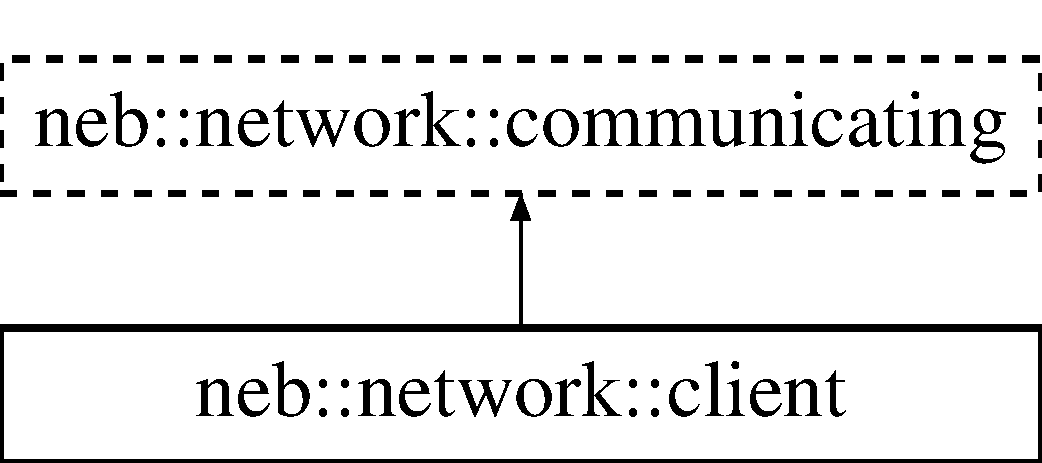
\includegraphics[height=2cm]{classneb_1_1network_1_1client}
\end{center}
\end{figure}
\subsection*{Public Member Functions}
\begin{DoxyCompactItemize}
\item 
\hypertarget{classneb_1_1network_1_1client_a4f117f86f1d548c492645b47ca3b1fb0}{
{\bfseries client} (neb::app\_\-s, char const $\ast$, unsigned short)}
\label{classneb_1_1network_1_1client_a4f117f86f1d548c492645b47ca3b1fb0}

\item 
\hypertarget{classneb_1_1network_1_1client_a04d1cdc645678b66a0c0bdfcf9eb3c1d}{
void {\bfseries process} (gal::network::message::shared\_\-t)}
\label{classneb_1_1network_1_1client_a04d1cdc645678b66a0c0bdfcf9eb3c1d}

\end{DoxyCompactItemize}


The documentation for this class was generated from the following files:\begin{DoxyCompactItemize}
\item 
src/nebula/network/client.hpp\item 
src/nebula/network/client.cpp\end{DoxyCompactItemize}

\hypertarget{classneb_1_1network_1_1communicating}{
\section{neb::network::communicating Class Reference}
\label{classneb_1_1network_1_1communicating}\index{neb::network::communicating@{neb::network::communicating}}
}
Inheritance diagram for neb::network::communicating::\begin{figure}[H]
\begin{center}
\leavevmode
\includegraphics[height=2cm]{classneb_1_1network_1_1communicating}
\end{center}
\end{figure}
\subsection*{Public Member Functions}
\begin{DoxyCompactItemize}
\item 
\hypertarget{classneb_1_1network_1_1communicating_aa56d7ee8b8546ecc25b2cc63603184e9}{
{\bfseries communicating} (neb::app\_\-s, int)}
\label{classneb_1_1network_1_1communicating_aa56d7ee8b8546ecc25b2cc63603184e9}

\item 
\hypertarget{classneb_1_1network_1_1communicating_a98c549330850584cd5ec57028785b777}{
void {\bfseries process} (gal::network::message::shared\_\-t)}
\label{classneb_1_1network_1_1communicating_a98c549330850584cd5ec57028785b777}

\end{DoxyCompactItemize}
\subsection*{Public Attributes}
\begin{DoxyCompactItemize}
\item 
\hypertarget{classneb_1_1network_1_1communicating_a9bac744763987c357b07a070ce2f1215}{
neb::app\_\-w {\bfseries app\_\-}}
\label{classneb_1_1network_1_1communicating_a9bac744763987c357b07a070ce2f1215}

\end{DoxyCompactItemize}


The documentation for this class was generated from the following files:\begin{DoxyCompactItemize}
\item 
src/nebula/network/communicating.hpp\item 
src/nebula/network/communicating.cpp\end{DoxyCompactItemize}

\hypertarget{classneb_1_1control_1_1rigid__body_1_1control}{\section{neb\-:\-:control\-:\-:rigid\-\_\-body\-:\-:control \-Class \-Reference}
\label{classneb_1_1control_1_1rigid__body_1_1control}\index{neb\-::control\-::rigid\-\_\-body\-::control@{neb\-::control\-::rigid\-\_\-body\-::control}}
}


\-Rigid \-Body \-An object (what did \-I mean by 'object' here, an actor?) makes no distinction between local and remote. \-In a remote scene, the actor will send a control update message. \-In a local scene, the actor will call upon stored values; it makes no difference to the actor whether these value were set by calls to key\-\_\-fun or by a control update message. \-This creates requirements for how control works. \-All infomation needed to determine force and torque at a given point in time must be stored in raw.  




{\ttfamily \#include $<$control.\-hpp$>$}

\subsection*{\-Public \-Member \-Functions}
\begin{DoxyCompactItemize}
\item 
\hypertarget{classneb_1_1control_1_1rigid__body_1_1control_a66fc3682afd8f4a94ccd241cb3ddddb3}{virtual int {\bfseries key\-\_\-fun} (int, int, int, int)}\label{classneb_1_1control_1_1rigid__body_1_1control_a66fc3682afd8f4a94ccd241cb3ddddb3}

\item 
\hypertarget{classneb_1_1control_1_1rigid__body_1_1control_a0649203ba08991125250be485dad9308}{void {\bfseries step\-\_\-local} (double)}\label{classneb_1_1control_1_1rigid__body_1_1control_a0649203ba08991125250be485dad9308}

\item 
\hypertarget{classneb_1_1control_1_1rigid__body_1_1control_a347b217d2133bf301aa9f31e084ccd6a}{void {\bfseries step\-\_\-local0} (double)}\label{classneb_1_1control_1_1rigid__body_1_1control_a347b217d2133bf301aa9f31e084ccd6a}

\item 
\hypertarget{classneb_1_1control_1_1rigid__body_1_1control_a6fad3693d3a31440201a928bc04e71d4}{void {\bfseries step\-\_\-local1} (double)}\label{classneb_1_1control_1_1rigid__body_1_1control_a6fad3693d3a31440201a928bc04e71d4}

\item 
\hypertarget{classneb_1_1control_1_1rigid__body_1_1control_aeaae8332076304e32a811e6f06410e18}{math\-::vec3$<$ double $>$ {\bfseries f} ()}\label{classneb_1_1control_1_1rigid__body_1_1control_aeaae8332076304e32a811e6f06410e18}

\item 
\hypertarget{classneb_1_1control_1_1rigid__body_1_1control_a0f2f5f0c00acbf26b2ae23c1db70f1d9}{math\-::vec3$<$ double $>$ {\bfseries t} ()}\label{classneb_1_1control_1_1rigid__body_1_1control_a0f2f5f0c00acbf26b2ae23c1db70f1d9}

\item 
\hypertarget{classneb_1_1control_1_1rigid__body_1_1control_a13cbe1e4aa9e9cbd38cc2424526779a3}{void {\bfseries print} ()}\label{classneb_1_1control_1_1rigid__body_1_1control_a13cbe1e4aa9e9cbd38cc2424526779a3}

\end{DoxyCompactItemize}
\subsection*{\-Public \-Attributes}
\begin{DoxyCompactItemize}
\item 
\hypertarget{classneb_1_1control_1_1rigid__body_1_1control_a5a8dc4754c9d46b288a468e0033af474}{neb\-::actor\-::\-Base\-\_\-w {\bfseries actor\-\_\-}}\label{classneb_1_1control_1_1rigid__body_1_1control_a5a8dc4754c9d46b288a468e0033af474}

\item 
\hypertarget{classneb_1_1control_1_1rigid__body_1_1control_a4a547bcc332479f91eecfcbaccfcb1c2}{\hyperlink{classneb_1_1control_1_1rigid__body_1_1raw}{neb\-::control\-::rigid\-\_\-body\-::raw} {\bfseries raw\-\_\-}}\label{classneb_1_1control_1_1rigid__body_1_1control_a4a547bcc332479f91eecfcbaccfcb1c2}

\item 
\hypertarget{classneb_1_1control_1_1rigid__body_1_1control_a5209e25d3b03696cd84710f34c991dea}{\begin{tabbing}
xx\=xx\=xx\=xx\=xx\=xx\=xx\=xx\=xx\=\kill
struct \{\\
\>key\_fun\_c {\bfseries key\_fun\_}\\
\} {\bfseries conn\_}}\label{classneb_1_1control_1_1rigid__body_1_1control_a5209e25d3b03696cd84710f34c991dea}
\\

\end{tabbing}\item 
\hypertarget{classneb_1_1control_1_1rigid__body_1_1control_a621b7abb234dfeae7db854a70899a96f}{gal\-::control\-::control {\bfseries pid\-\_\-}}\label{classneb_1_1control_1_1rigid__body_1_1control_a621b7abb234dfeae7db854a70899a96f}

\item 
\hypertarget{classneb_1_1control_1_1rigid__body_1_1control_a15a9bb7db7b5d2b8dc8d99a3bff00d68}{double {\bfseries last\-\_\-}}\label{classneb_1_1control_1_1rigid__body_1_1control_a15a9bb7db7b5d2b8dc8d99a3bff00d68}

\end{DoxyCompactItemize}


\subsection{\-Detailed \-Description}
\-Rigid \-Body \-An object (what did \-I mean by 'object' here, an actor?) makes no distinction between local and remote. \-In a remote scene, the actor will send a control update message. \-In a local scene, the actor will call upon stored values; it makes no difference to the actor whether these value were set by calls to key\-\_\-fun or by a control update message. \-This creates requirements for how control works. \-All infomation needed to determine force and torque at a given point in time must be stored in raw. 

\-The documentation for this class was generated from the following files\-:\begin{DoxyCompactItemize}
\item 
src/nebula/control/rigid\-\_\-body/control.\-hpp\item 
src/nebula/control/rigid\-\_\-body/control.\-cpp\end{DoxyCompactItemize}

\hypertarget{classneb_1_1Actor_1_1Controller}{\section{neb\-:\-:\-Actor\-:\-:\-Controller \-Class \-Reference}
\label{classneb_1_1Actor_1_1Controller}\index{neb\-::\-Actor\-::\-Controller@{neb\-::\-Actor\-::\-Controller}}
}
\-Inheritance diagram for neb\-:\-:\-Actor\-:\-:\-Controller\-:\begin{figure}[H]
\begin{center}
\leavevmode
\includegraphics[height=2.000000cm]{classneb_1_1Actor_1_1Controller}
\end{center}
\end{figure}
\subsection*{\-Public \-Member \-Functions}
\begin{DoxyCompactItemize}
\item 
\hypertarget{classneb_1_1Actor_1_1Controller_aeedad5d671d8d4bc4398efd7be7fc005}{{\bfseries \-Controller} (glutpp\-::actor\-::parent\-\_\-s)}\label{classneb_1_1Actor_1_1Controller_aeedad5d671d8d4bc4398efd7be7fc005}

\item 
\hypertarget{classneb_1_1Actor_1_1Controller_ac6f5996da2aea174de794de4ffc647f4}{virtual void {\bfseries release} ()}\label{classneb_1_1Actor_1_1Controller_ac6f5996da2aea174de794de4ffc647f4}

\item 
\hypertarget{classneb_1_1Actor_1_1Controller_a95830d761987167e8ab122f3ca16346f}{virtual void {\bfseries step} (float)}\label{classneb_1_1Actor_1_1Controller_a95830d761987167e8ab122f3ca16346f}

\item 
\hypertarget{classneb_1_1Actor_1_1Controller_aad1420da60579f17c8dec8dad2a517bb}{virtual void {\bfseries init} (glutpp\-::actor\-::desc\-\_\-s)}\label{classneb_1_1Actor_1_1Controller_aad1420da60579f17c8dec8dad2a517bb}

\item 
\hypertarget{classneb_1_1Actor_1_1Controller_ab8ab78f513b014f112895de7dad43040}{virtual void {\bfseries add\-\_\-force} ()}\label{classneb_1_1Actor_1_1Controller_ab8ab78f513b014f112895de7dad43040}

\end{DoxyCompactItemize}
\subsection*{\-Public \-Attributes}
\begin{DoxyCompactItemize}
\item 
\hypertarget{classneb_1_1Actor_1_1Controller_aa692b62e071660a4e182406efb10272b}{physx\-::\-Px\-Controller $\ast$ {\bfseries px\-\_\-controller\-\_\-}}\label{classneb_1_1Actor_1_1Controller_aa692b62e071660a4e182406efb10272b}

\end{DoxyCompactItemize}


\-The documentation for this class was generated from the following files\-:\begin{DoxyCompactItemize}
\item 
src/nebula/actor/\-Controller.\-hpp\item 
src/nebula/actor/\-Controller.\-cpp\end{DoxyCompactItemize}

\hypertarget{classneb_1_1network_1_1control_1_1rigid__body_1_1create}{\section{neb\-:\-:network\-:\-:control\-:\-:rigid\-\_\-body\-:\-:create \-Class \-Reference}
\label{classneb_1_1network_1_1control_1_1rigid__body_1_1create}\index{neb\-::network\-::control\-::rigid\-\_\-body\-::create@{neb\-::network\-::control\-::rigid\-\_\-body\-::create}}
}
\subsection*{\-Public \-Member \-Functions}
\begin{DoxyCompactItemize}
\item 
\hypertarget{classneb_1_1network_1_1control_1_1rigid__body_1_1create_af3941f85f8c8499440492a4b4373231f}{glutpp\-::actor\-::addr\-\_\-s {\bfseries get\-\_\-addr} ()}\label{classneb_1_1network_1_1control_1_1rigid__body_1_1create_af3941f85f8c8499440492a4b4373231f}

\end{DoxyCompactItemize}


\-The documentation for this class was generated from the following file\-:\begin{DoxyCompactItemize}
\item 
src/nebula/network/message.\-hpp\end{DoxyCompactItemize}

\hypertarget{classDefaultErrorCallback}{
\section{DefaultErrorCallback Class Reference}
\label{classDefaultErrorCallback}\index{DefaultErrorCallback@{DefaultErrorCallback}}
}
\subsection*{Public Member Functions}
\begin{DoxyCompactItemize}
\item 
\hypertarget{classDefaultErrorCallback_ae95118f6a45b47a1b72af9417f80d84e}{
void {\bfseries reportError} (physx::PxErrorCode::Enum code, char const $\ast$message, char const $\ast$file, int line)}
\label{classDefaultErrorCallback_ae95118f6a45b47a1b72af9417f80d84e}

\end{DoxyCompactItemize}


The documentation for this class was generated from the following files:\begin{DoxyCompactItemize}
\item 
src/nebula/physics.hpp\item 
src/nebula/physics.cpp\end{DoxyCompactItemize}

\hypertarget{classneb_1_1Actor_1_1empty}{\section{neb\-:\-:\-Actor\-:\-:empty \-Class \-Reference}
\label{classneb_1_1Actor_1_1empty}\index{neb\-::\-Actor\-::empty@{neb\-::\-Actor\-::empty}}
}


\-Inheritance diagram for neb\-:\-:\-Actor\-:\-:empty\-:\nopagebreak
\begin{figure}[H]
\begin{center}
\leavevmode
\includegraphics[width=350pt]{classneb_1_1Actor_1_1empty__inherit__graph}
\end{center}
\end{figure}


\-Collaboration diagram for neb\-:\-:\-Actor\-:\-:empty\-:\nopagebreak
\begin{figure}[H]
\begin{center}
\leavevmode
\includegraphics[width=350pt]{classneb_1_1Actor_1_1empty__coll__graph}
\end{center}
\end{figure}
\subsection*{\-Public \-Member \-Functions}
\begin{DoxyCompactItemize}
\item 
\hypertarget{classneb_1_1Actor_1_1empty_ac9892c883ff1ad7b22ec43142d18f9e9}{{\bfseries empty} (\hyperlink{classNeb_1_1weak__ptr}{\-Neb\-::\-Actor\-::parent\-\_\-w})}\label{classneb_1_1Actor_1_1empty_ac9892c883ff1ad7b22ec43142d18f9e9}

\item 
\hypertarget{classneb_1_1Actor_1_1empty_adef9eaa1dfbc51f1be6acd3b480ee27a}{virtual void {\bfseries init} (\hyperlink{classNeb_1_1weak__ptr}{\-Neb\-::\-Actor\-::desc\-\_\-w})}\label{classneb_1_1Actor_1_1empty_adef9eaa1dfbc51f1be6acd3b480ee27a}

\item 
\hypertarget{classneb_1_1Actor_1_1empty_a473dcef1b8de90a5178e506406e5f383}{virtual void {\bfseries add\-\_\-force} (double)}\label{classneb_1_1Actor_1_1empty_a473dcef1b8de90a5178e506406e5f383}

\item 
\hypertarget{classneb_1_1Actor_1_1empty_ab1ab81960ecca1bf3f2410906cdee3e1}{virtual void {\bfseries create\-\_\-physics} ()}\label{classneb_1_1Actor_1_1empty_ab1ab81960ecca1bf3f2410906cdee3e1}

\item 
\hypertarget{classneb_1_1Actor_1_1empty_aa0e380242b5613196fe6d1dac5cb6b4d}{virtual void {\bfseries init\-\_\-physics} ()}\label{classneb_1_1Actor_1_1empty_aa0e380242b5613196fe6d1dac5cb6b4d}

\end{DoxyCompactItemize}


\-The documentation for this class was generated from the following files\-:\begin{DoxyCompactItemize}
\item 
src/\-Nebula/\-Actor/empty.\-hpp\item 
src/\-Nebula/\-Actor/empty.\-cpp\end{DoxyCompactItemize}

\hypertarget{structneb_1_1app_1_1flag}{
\section{neb::app::flag Struct Reference}
\label{structneb_1_1app_1_1flag}\index{neb::app::flag@{neb::app::flag}}
}
\subsection*{Public Types}
\begin{DoxyCompactItemize}
\item 
enum {\bfseries e} \{ {\bfseries SHOULD\_\-RELEASE} =  1 $<$$<$ 0
 \}
\end{DoxyCompactItemize}


The documentation for this struct was generated from the following file:\begin{DoxyCompactItemize}
\item 
src/nebula/app.hpp\end{DoxyCompactItemize}

\hypertarget{classneb_1_1geometry}{\section{neb\-:\-:geometry \-Class \-Reference}
\label{classneb_1_1geometry}\index{neb\-::geometry@{neb\-::geometry}}
}
\subsection*{\-Public \-Types}
\begin{DoxyCompactItemize}
\item 
enum {\bfseries type} \{ {\bfseries \-B\-O\-X}, 
{\bfseries \-S\-P\-H\-E\-R\-E}
 \}
\end{DoxyCompactItemize}
\subsection*{\-Public \-Attributes}
\begin{DoxyCompactItemize}
\item 
\hypertarget{classneb_1_1geometry_a5747e38891f27136cd45a23ea986b595}{type {\bfseries type\-\_\-}}\label{classneb_1_1geometry_a5747e38891f27136cd45a23ea986b595}

\item 
\hypertarget{classneb_1_1geometry_a2e7f1ef07f66b904852c1ae9e84f9f55}{physx\-::\-Px\-Geometry $\ast$ {\bfseries geo\-\_\-}}\label{classneb_1_1geometry_a2e7f1ef07f66b904852c1ae9e84f9f55}

\end{DoxyCompactItemize}


\-The documentation for this class was generated from the following file\-:\begin{DoxyCompactItemize}
\item 
src/nebula/actor/geometry.\-hpp\end{DoxyCompactItemize}

\hypertarget{classneb_1_1physics}{
\section{neb::physics Class Reference}
\label{classneb_1_1physics}\index{neb::physics@{neb::physics}}
}
\subsection*{Public Member Functions}
\begin{DoxyCompactItemize}
\item 
\hypertarget{classneb_1_1physics_a43cb026789894c6dda3657f83a2cb8d1}{
void {\bfseries Init} ()}
\label{classneb_1_1physics_a43cb026789894c6dda3657f83a2cb8d1}

\item 
\hypertarget{classneb_1_1physics_a24efe8826dbb2b6fa42ee21360123834}{
void {\bfseries Shutdown} ()}
\label{classneb_1_1physics_a24efe8826dbb2b6fa42ee21360123834}

\end{DoxyCompactItemize}
\subsection*{Public Attributes}
\begin{DoxyCompactItemize}
\item 
\hypertarget{classneb_1_1physics_a819d98df4d7357116516e0f2df0e34fc}{
\hyperlink{classDefaultErrorCallback}{DefaultErrorCallback} {\bfseries px\_\-default\_\-error\_\-callback\_\-}}
\label{classneb_1_1physics_a819d98df4d7357116516e0f2df0e34fc}

\item 
\hypertarget{classneb_1_1physics_a63bea60198e1c6460c104fdd38ab2018}{
physx::PxDefaultAllocator {\bfseries px\_\-default\_\-allocator\_\-callback\_\-}}
\label{classneb_1_1physics_a63bea60198e1c6460c104fdd38ab2018}

\item 
\hypertarget{classneb_1_1physics_ab6ad04fa0dd429d2e43808dbe4ff6874}{
physx::PxFoundation $\ast$ {\bfseries px\_\-foundation\_\-}}
\label{classneb_1_1physics_ab6ad04fa0dd429d2e43808dbe4ff6874}

\item 
\hypertarget{classneb_1_1physics_afc65796d459735ca9e946582934f57ad}{
physx::PxPhysics $\ast$ {\bfseries px\_\-physics\_\-}}
\label{classneb_1_1physics_afc65796d459735ca9e946582934f57ad}

\item 
\hypertarget{classneb_1_1physics_a727d7d7cb92e32a99d3b3463993f989f}{
physx::PxProfileZoneManager $\ast$ {\bfseries px\_\-profile\_\-zone\_\-manager\_\-}}
\label{classneb_1_1physics_a727d7d7cb92e32a99d3b3463993f989f}

\item 
\hypertarget{classneb_1_1physics_ab12401759700525d86a7219d6c649e7b}{
physx::PxCooking $\ast$ {\bfseries px\_\-cooking\_\-}}
\label{classneb_1_1physics_ab12401759700525d86a7219d6c649e7b}

\item 
\hypertarget{classneb_1_1physics_aa7129bf5f326d56721c401780fab8613}{
physx::pxtask::CudaContextManager $\ast$ {\bfseries px\_\-cuda\_\-context\_\-manager\_\-}}
\label{classneb_1_1physics_aa7129bf5f326d56721c401780fab8613}

\item 
\hypertarget{classneb_1_1physics_ab736a4b3ffe77be9ef6be2ea128fcaf8}{
physx::PxControllerManager $\ast$ {\bfseries px\_\-character\_\-controller\_\-manager\_\-}}
\label{classneb_1_1physics_ab736a4b3ffe77be9ef6be2ea128fcaf8}

\end{DoxyCompactItemize}


The documentation for this class was generated from the following files:\begin{DoxyCompactItemize}
\item 
src/nebula/physics.hpp\item 
src/nebula/physics.cpp\end{DoxyCompactItemize}

\hypertarget{classneb_1_1Actor_1_1raw}{\section{neb\-:\-:\-Actor\-:\-:raw \-Class \-Reference}
\label{classneb_1_1Actor_1_1raw}\index{neb\-::\-Actor\-::raw@{neb\-::\-Actor\-::raw}}
}
\subsection*{\-Public \-Member \-Functions}
\begin{DoxyCompactItemize}
\item 
\hypertarget{classneb_1_1Actor_1_1raw_a7940b6e04d8edb718757d763635ded88}{virtual void {\bfseries load} (tinyxml2\-::\-X\-M\-L\-Element $\ast$)}\label{classneb_1_1Actor_1_1raw_a7940b6e04d8edb718757d763635ded88}

\item 
\hypertarget{classneb_1_1Actor_1_1raw_a2c77b67b8525fd5ead9966c1e00b58aa}{virtual void {\bfseries load} (glutpp\-::actor\-::actor\-\_\-s)}\label{classneb_1_1Actor_1_1raw_a2c77b67b8525fd5ead9966c1e00b58aa}

\end{DoxyCompactItemize}
\subsection*{\-Public \-Attributes}
\begin{DoxyCompactItemize}
\item 
\hypertarget{classneb_1_1Actor_1_1raw_af2cd08be96aafc52e7c43c588cd7bddf}{float {\bfseries health\-\_\-}}\label{classneb_1_1Actor_1_1raw_af2cd08be96aafc52e7c43c588cd7bddf}

\end{DoxyCompactItemize}
\subsection*{\-Friends}
\begin{DoxyCompactItemize}
\item 
\hypertarget{classneb_1_1Actor_1_1raw_ae5367c8b565cf6a910d5822eab22d2d9}{class {\bfseries neb\-::\-Actor\-::raw\-\_\-factory}}\label{classneb_1_1Actor_1_1raw_ae5367c8b565cf6a910d5822eab22d2d9}

\item 
\hypertarget{classneb_1_1Actor_1_1raw_a89c753bf1646b22d579368032648a476}{void {\bfseries gal\-::reset} (neb\-::\-Actor\-::raw\-\_\-s \&)}\label{classneb_1_1Actor_1_1raw_a89c753bf1646b22d579368032648a476}

\end{DoxyCompactItemize}


\-The documentation for this class was generated from the following file\-:\begin{DoxyCompactItemize}
\item 
src/nebula/actor/raw.\-hpp\end{DoxyCompactItemize}

\hypertarget{classneb_1_1control_1_1rigid__body_1_1raw}{\section{neb\-:\-:control\-:\-:rigid\-\_\-body\-:\-:raw \-Class \-Reference}
\label{classneb_1_1control_1_1rigid__body_1_1raw}\index{neb\-::control\-::rigid\-\_\-body\-::raw@{neb\-::control\-::rigid\-\_\-body\-::raw}}
}
\subsection*{\-Public \-Member \-Functions}
\begin{DoxyCompactItemize}
\item 
\hypertarget{classneb_1_1control_1_1rigid__body_1_1raw_a79de740ae20967e3e3e3139c85766f41}{void {\bfseries load} (neb\-::control\-::rigid\-\_\-body\-::control\-\_\-s)}\label{classneb_1_1control_1_1rigid__body_1_1raw_a79de740ae20967e3e3e3139c85766f41}

\end{DoxyCompactItemize}
\subsection*{\-Public \-Attributes}
\begin{DoxyCompactItemize}
\item 
\hypertarget{classneb_1_1control_1_1rigid__body_1_1raw_a8f5fb347a6c58f62b223c48a1813e2e4}{type {\bfseries type\-\_\-}}\label{classneb_1_1control_1_1rigid__body_1_1raw_a8f5fb347a6c58f62b223c48a1813e2e4}

\item 
\hypertarget{classneb_1_1control_1_1rigid__body_1_1raw_a472812f3800fc91527720e7922aa11f7}{math\-::quat {\bfseries q\-\_\-target\-\_\-}}\label{classneb_1_1control_1_1rigid__body_1_1raw_a472812f3800fc91527720e7922aa11f7}

\item 
\hypertarget{classneb_1_1control_1_1rigid__body_1_1raw_a65f9cf9ce195cef108adfdfca2f94478}{math\-::vec3$<$ double $>$ {\bfseries p\-\_\-target\-\_\-}}\label{classneb_1_1control_1_1rigid__body_1_1raw_a65f9cf9ce195cef108adfdfca2f94478}

\item 
\hypertarget{classneb_1_1control_1_1rigid__body_1_1raw_a1af8a9c496392f96a542964536a41f1f}{math\-::vec3$<$ double $>$ {\bfseries f\-\_\-}}\label{classneb_1_1control_1_1rigid__body_1_1raw_a1af8a9c496392f96a542964536a41f1f}

\item 
\hypertarget{classneb_1_1control_1_1rigid__body_1_1raw_a5a5814c383407852a180a03451aab534}{math\-::vec3$<$ double $>$ {\bfseries t\-\_\-}}\label{classneb_1_1control_1_1rigid__body_1_1raw_a5a5814c383407852a180a03451aab534}

\item 
\hypertarget{classneb_1_1control_1_1rigid__body_1_1raw_aa4ce0e8f719757e560c259b015f35200}{math\-::vec3$<$ double $>$ {\bfseries force\-\_\-}}\label{classneb_1_1control_1_1rigid__body_1_1raw_aa4ce0e8f719757e560c259b015f35200}

\item 
\hypertarget{classneb_1_1control_1_1rigid__body_1_1raw_aff9ff856531641609a94713bda40fef9}{math\-::vec3$<$ double $>$ {\bfseries torque\-\_\-}}\label{classneb_1_1control_1_1rigid__body_1_1raw_aff9ff856531641609a94713bda40fef9}

\end{DoxyCompactItemize}


\-The documentation for this class was generated from the following files\-:\begin{DoxyCompactItemize}
\item 
src/nebula/control/rigid\-\_\-body/raw.\-hpp\item 
src/nebula/actor/raw.\-cpp\item 
src/nebula/control/rigid\-\_\-body/raw.\-cpp\end{DoxyCompactItemize}

\hypertarget{classneb_1_1actor_1_1raw__factory}{
\section{neb::actor::raw\_\-factory Class Reference}
\label{classneb_1_1actor_1_1raw__factory}\index{neb::actor::raw\_\-factory@{neb::actor::raw\_\-factory}}
}
\subsection*{Public Member Functions}
\begin{DoxyCompactItemize}
\item 
\hypertarget{classneb_1_1actor_1_1raw__factory_a2118b6982b4d59339bbb855e3beaaba9}{
virtual glutpp::actor::raw\_\-s {\bfseries create} (int)}
\label{classneb_1_1actor_1_1raw__factory_a2118b6982b4d59339bbb855e3beaaba9}

\end{DoxyCompactItemize}


The documentation for this class was generated from the following files:\begin{DoxyCompactItemize}
\item 
src/nebula/actor/raw\_\-factory.hpp\item 
src/nebula/actor/raw\_\-factory.cpp\end{DoxyCompactItemize}

\hypertarget{classneb_1_1Actor_1_1Rigid__Dynamic}{\section{neb\-:\-:\-Actor\-:\-:\-Rigid\-\_\-\-Dynamic \-Class \-Reference}
\label{classneb_1_1Actor_1_1Rigid__Dynamic}\index{neb\-::\-Actor\-::\-Rigid\-\_\-\-Dynamic@{neb\-::\-Actor\-::\-Rigid\-\_\-\-Dynamic}}
}
\-Inheritance diagram for neb\-:\-:\-Actor\-:\-:\-Rigid\-\_\-\-Dynamic\-:\begin{figure}[H]
\begin{center}
\leavevmode
\includegraphics[height=5.000000cm]{classneb_1_1Actor_1_1Rigid__Dynamic}
\end{center}
\end{figure}
\subsection*{\-Public \-Member \-Functions}
\begin{DoxyCompactItemize}
\item 
\hypertarget{classneb_1_1Actor_1_1Rigid__Dynamic_ab532d1a36c9b942caa1e136d274308f8}{{\bfseries \-Rigid\-\_\-\-Dynamic} (glutpp\-::actor\-::parent\-\_\-s)}\label{classneb_1_1Actor_1_1Rigid__Dynamic_ab532d1a36c9b942caa1e136d274308f8}

\item 
\hypertarget{classneb_1_1Actor_1_1Rigid__Dynamic_a8ed2e28125967f980bb55d5697ea5b81}{virtual void {\bfseries init} (glutpp\-::actor\-::desc\-\_\-s)}\label{classneb_1_1Actor_1_1Rigid__Dynamic_a8ed2e28125967f980bb55d5697ea5b81}

\item 
\hypertarget{classneb_1_1Actor_1_1Rigid__Dynamic_a22912f857b64132c4638e94a3454a801}{virtual void {\bfseries create\-\_\-physics} ()}\label{classneb_1_1Actor_1_1Rigid__Dynamic_a22912f857b64132c4638e94a3454a801}

\item 
\hypertarget{classneb_1_1Actor_1_1Rigid__Dynamic_a81bda0edf17d6b7ed7f0c807cc23cc33}{virtual void {\bfseries init\-\_\-physics} ()}\label{classneb_1_1Actor_1_1Rigid__Dynamic_a81bda0edf17d6b7ed7f0c807cc23cc33}

\item 
\hypertarget{classneb_1_1Actor_1_1Rigid__Dynamic_a20ebed0437aec0f1ad5ca0bb2c2edf4a}{virtual void {\bfseries print\-\_\-info} ()}\label{classneb_1_1Actor_1_1Rigid__Dynamic_a20ebed0437aec0f1ad5ca0bb2c2edf4a}

\end{DoxyCompactItemize}


\-The documentation for this class was generated from the following files\-:\begin{DoxyCompactItemize}
\item 
src/nebula/actor/\-Rigid\-\_\-\-Dynamic.\-hpp\item 
src/nebula/actor/\-Rigid\-\_\-\-Dynamic.\-cpp\end{DoxyCompactItemize}

\hypertarget{classneb_1_1actor_1_1Rigid__Dynamic__Box}{
\section{neb::actor::Rigid\_\-Dynamic\_\-Box Class Reference}
\label{classneb_1_1actor_1_1Rigid__Dynamic__Box}\index{neb::actor::Rigid\_\-Dynamic\_\-Box@{neb::actor::Rigid\_\-Dynamic\_\-Box}}
}
Inheritance diagram for neb::actor::Rigid\_\-Dynamic\_\-Box::\begin{figure}[H]
\begin{center}
\leavevmode
\includegraphics[height=6cm]{classneb_1_1actor_1_1Rigid__Dynamic__Box}
\end{center}
\end{figure}
\subsection*{Public Member Functions}
\begin{DoxyCompactItemize}
\item 
\hypertarget{classneb_1_1actor_1_1Rigid__Dynamic__Box_ad2564e54df3b07cc2454ba28a026b765}{
void {\bfseries Display} ()}
\label{classneb_1_1actor_1_1Rigid__Dynamic__Box_ad2564e54df3b07cc2454ba28a026b765}

\end{DoxyCompactItemize}


The documentation for this class was generated from the following file:\begin{DoxyCompactItemize}
\item 
src/nebula/actor/Rigid\_\-Dynamic\_\-Box.hpp\end{DoxyCompactItemize}

\hypertarget{classneb_1_1Actor_1_1Rigid__Static}{\section{neb\-:\-:\-Actor\-:\-:\-Rigid\-\_\-\-Static \-Class \-Reference}
\label{classneb_1_1Actor_1_1Rigid__Static}\index{neb\-::\-Actor\-::\-Rigid\-\_\-\-Static@{neb\-::\-Actor\-::\-Rigid\-\_\-\-Static}}
}
\subsection*{\-Public \-Member \-Functions}
\begin{DoxyCompactItemize}
\item 
\hypertarget{classneb_1_1Actor_1_1Rigid__Static_af50cb5d837b3e222c0171bce9a95131b}{{\bfseries \-Rigid\-\_\-\-Static} (boost\-::shared\-\_\-ptr$<$ glutpp\-::actor\-::parent $>$ parent)}\label{classneb_1_1Actor_1_1Rigid__Static_af50cb5d837b3e222c0171bce9a95131b}

\item 
\hypertarget{classneb_1_1Actor_1_1Rigid__Static_ac20c1721c784026a4ba9fae43a83f25e}{virtual void {\bfseries init} (boost\-::shared\-\_\-ptr$<$ glutpp\-::actor\-::desc $>$)}\label{classneb_1_1Actor_1_1Rigid__Static_ac20c1721c784026a4ba9fae43a83f25e}

\item 
\hypertarget{classneb_1_1Actor_1_1Rigid__Static_ac811bdd9fadf4cdc434ca8696e583f32}{virtual void {\bfseries create\-\_\-physics} ()}\label{classneb_1_1Actor_1_1Rigid__Static_ac811bdd9fadf4cdc434ca8696e583f32}

\item 
\hypertarget{classneb_1_1Actor_1_1Rigid__Static_a21b5c36de8bc1b6d8ac3bf8ccf69c12d}{virtual void {\bfseries init\-\_\-physics} ()}\label{classneb_1_1Actor_1_1Rigid__Static_a21b5c36de8bc1b6d8ac3bf8ccf69c12d}

\item 
\hypertarget{classneb_1_1Actor_1_1Rigid__Static_af8a2758eb88f3e0d8f7faff3d0e536bb}{virtual void {\bfseries step\-\_\-local} (double)}\label{classneb_1_1Actor_1_1Rigid__Static_af8a2758eb88f3e0d8f7faff3d0e536bb}

\item 
\hypertarget{classneb_1_1Actor_1_1Rigid__Static_a1fbb2f59383d23142dc6fcdd8204fafe}{virtual void {\bfseries step\-\_\-remote} (double)}\label{classneb_1_1Actor_1_1Rigid__Static_a1fbb2f59383d23142dc6fcdd8204fafe}

\end{DoxyCompactItemize}


\-The documentation for this class was generated from the following files\-:\begin{DoxyCompactItemize}
\item 
src/\-Nebula/\-Actor/\-Rigid\-\_\-\-Static.\-hpp\item 
src/\-Nebula/\-Actor/\-Rigid\-\_\-\-Static.\-cpp\end{DoxyCompactItemize}

\hypertarget{classneb_1_1Actor_1_1RigidActor}{
\section{neb::Actor::RigidActor Class Reference}
\label{classneb_1_1Actor_1_1RigidActor}\index{neb::Actor::RigidActor@{neb::Actor::RigidActor}}
}
\subsection*{Public Member Functions}
\begin{DoxyCompactItemize}
\item 
\hypertarget{classneb_1_1Actor_1_1RigidActor_aa253e1971cdd1f4b3ddef3fe1fe7f863}{
{\bfseries RigidActor} (glutpp::actor::parent\_\-s)}
\label{classneb_1_1Actor_1_1RigidActor_aa253e1971cdd1f4b3ddef3fe1fe7f863}

\item 
\hypertarget{classneb_1_1Actor_1_1RigidActor_a967e256371080add564411b51b94f297}{
virtual void {\bfseries init} (glutpp::actor::desc\_\-s)}
\label{classneb_1_1Actor_1_1RigidActor_a967e256371080add564411b51b94f297}

\item 
\hypertarget{classneb_1_1Actor_1_1RigidActor_aa46996a108d191eaa0c05beabe8ba015}{
virtual void {\bfseries add\_\-force} (double)}
\label{classneb_1_1Actor_1_1RigidActor_aa46996a108d191eaa0c05beabe8ba015}

\item 
\hypertarget{classneb_1_1Actor_1_1RigidActor_a329821fb69766e1c33834885e6634555}{
virtual void {\bfseries step\_\-local} (double)}
\label{classneb_1_1Actor_1_1RigidActor_a329821fb69766e1c33834885e6634555}

\item 
\hypertarget{classneb_1_1Actor_1_1RigidActor_a072ffe441731d0709f14a3785371e860}{
virtual void {\bfseries step\_\-remote} (double)}
\label{classneb_1_1Actor_1_1RigidActor_a072ffe441731d0709f14a3785371e860}

\item 
\hypertarget{classneb_1_1Actor_1_1RigidActor_a6007e808c5437eafdf7fe8a76878c0cb}{
virtual void {\bfseries setupFiltering} ()}
\label{classneb_1_1Actor_1_1RigidActor_a6007e808c5437eafdf7fe8a76878c0cb}

\item 
\hypertarget{classneb_1_1Actor_1_1RigidActor_ab548e314daab07a821783a84cd072992}{
virtual glutpp::actor::desc\_\-s {\bfseries get\_\-projectile} ()}
\label{classneb_1_1Actor_1_1RigidActor_ab548e314daab07a821783a84cd072992}

\item 
\hypertarget{classneb_1_1Actor_1_1RigidActor_ae43181ba4f6b5b3fb782f6a689ec5dc5}{
virtual void {\bfseries create\_\-physics} ()}
\label{classneb_1_1Actor_1_1RigidActor_ae43181ba4f6b5b3fb782f6a689ec5dc5}

\item 
\hypertarget{classneb_1_1Actor_1_1RigidActor_a558079bb45a9986bfbfcb92c2d8e005a}{
virtual void {\bfseries init\_\-physics} ()}
\label{classneb_1_1Actor_1_1RigidActor_a558079bb45a9986bfbfcb92c2d8e005a}

\item 
\hypertarget{classneb_1_1Actor_1_1RigidActor_a584f596160a4b44a1ddc6cc24b405d04}{
virtual void {\bfseries print\_\-info} ()}
\label{classneb_1_1Actor_1_1RigidActor_a584f596160a4b44a1ddc6cc24b405d04}

\end{DoxyCompactItemize}


The documentation for this class was generated from the following file:\begin{DoxyCompactItemize}
\item 
src/nebula/actor/Rigid\_\-Actor.hpp\end{DoxyCompactItemize}

\hypertarget{classneb_1_1Actor_1_1RigidBody_1_1RigidBody}{\section{neb\-:\-:\-Actor\-:\-:\-Rigid\-Body\-:\-:\-Rigid\-Body \-Class \-Reference}
\label{classneb_1_1Actor_1_1RigidBody_1_1RigidBody}\index{neb\-::\-Actor\-::\-Rigid\-Body\-::\-Rigid\-Body@{neb\-::\-Actor\-::\-Rigid\-Body\-::\-Rigid\-Body}}
}
\-Inheritance diagram for neb\-:\-:\-Actor\-:\-:\-Rigid\-Body\-:\-:\-Rigid\-Body\-:\begin{figure}[H]
\begin{center}
\leavevmode
\includegraphics[height=5.000000cm]{classneb_1_1Actor_1_1RigidBody_1_1RigidBody}
\end{center}
\end{figure}
\subsection*{\-Public \-Member \-Functions}
\begin{DoxyCompactItemize}
\item 
\hypertarget{classneb_1_1Actor_1_1RigidBody_1_1RigidBody_a4a42b50cdc34ed40704fe68a6044aac5}{{\bfseries \-Rigid\-Body} (glutpp\-::actor\-::parent\-\_\-s)}\label{classneb_1_1Actor_1_1RigidBody_1_1RigidBody_a4a42b50cdc34ed40704fe68a6044aac5}

\item 
\hypertarget{classneb_1_1Actor_1_1RigidBody_1_1RigidBody_a49bc7986eea3d48486dc8bdba8b84954}{virtual void {\bfseries init} (glutpp\-::actor\-::desc\-\_\-s)}\label{classneb_1_1Actor_1_1RigidBody_1_1RigidBody_a49bc7986eea3d48486dc8bdba8b84954}

\item 
\hypertarget{classneb_1_1Actor_1_1RigidBody_1_1RigidBody_af9d4be08596daf414fc020ac6c659a6e}{virtual glutpp\-::actor\-::desc\-\_\-s {\bfseries get\-\_\-projectile} ()}\label{classneb_1_1Actor_1_1RigidBody_1_1RigidBody_af9d4be08596daf414fc020ac6c659a6e}

\item 
\hypertarget{classneb_1_1Actor_1_1RigidBody_1_1RigidBody_a113a8004e1564ce207c89101bb015086}{virtual void {\bfseries print\-\_\-info} ()}\label{classneb_1_1Actor_1_1RigidBody_1_1RigidBody_a113a8004e1564ce207c89101bb015086}

\item 
\hypertarget{classneb_1_1Actor_1_1RigidBody_1_1RigidBody_a690d134f35e34636883622d13596592c}{virtual void {\bfseries create\-\_\-physics} ()}\label{classneb_1_1Actor_1_1RigidBody_1_1RigidBody_a690d134f35e34636883622d13596592c}

\item 
\hypertarget{classneb_1_1Actor_1_1RigidBody_1_1RigidBody_a5217679a926c4bdbd9006545751c39ac}{virtual void {\bfseries create\-\_\-control} (neb\-::control\-::rigid\-\_\-body\-::raw\-\_\-s)}\label{classneb_1_1Actor_1_1RigidBody_1_1RigidBody_a5217679a926c4bdbd9006545751c39ac}

\end{DoxyCompactItemize}
\subsection*{\-Public \-Attributes}
\begin{DoxyCompactItemize}
\item 
\hypertarget{classneb_1_1Actor_1_1RigidBody_1_1RigidBody_a873b6a4d9a88f20b12cbae77aeed5607}{neb\-::control\-::rigid\-\_\-body\-::control\-\_\-s {\bfseries control\-\_\-}}\label{classneb_1_1Actor_1_1RigidBody_1_1RigidBody_a873b6a4d9a88f20b12cbae77aeed5607}

\end{DoxyCompactItemize}


\-The documentation for this class was generated from the following file\-:\begin{DoxyCompactItemize}
\item 
src/nebula/actor/rigid\-\_\-body/rigid\-\_\-body.\-hpp\end{DoxyCompactItemize}

\hypertarget{classneb_1_1scene_1_1scene}{
\section{neb::scene::scene Class Reference}
\label{classneb_1_1scene_1_1scene}\index{neb::scene::scene@{neb::scene::scene}}
}
\subsection*{Public Types}
\begin{DoxyCompactItemize}
\item 
enum \{ {\bfseries NONE} =  0, 
{\bfseries LOCAL}, 
{\bfseries REMOTE}
 \}
\item 
\hypertarget{classneb_1_1scene_1_1scene_a12a166d302ebe2c0ccc39c97d8dcd58b}{
typedef std::shared\_\-ptr$<$ neb::actor::Base $>$ {\bfseries base\_\-t}}
\label{classneb_1_1scene_1_1scene_a12a166d302ebe2c0ccc39c97d8dcd58b}

\item 
\hypertarget{classneb_1_1scene_1_1scene_a102a6dc3de38eda425650b9122676a78}{
typedef std::shared\_\-ptr$<$ \hyperlink{classneb_1_1actor_1_1Rigid__Dynamic}{neb::actor::Rigid\_\-Dynamic} $>$ {\bfseries rigid\_\-dynamic\_\-t}}
\label{classneb_1_1scene_1_1scene_a102a6dc3de38eda425650b9122676a78}

\item 
\hypertarget{classneb_1_1scene_1_1scene_a782cb687dc9d61c8fcd5b12aa4189487}{
typedef std::shared\_\-ptr$<$ \hyperlink{classneb_1_1actor_1_1Rigid__Static}{neb::actor::Rigid\_\-Static} $>$ {\bfseries rigid\_\-static\_\-t}}
\label{classneb_1_1scene_1_1scene_a782cb687dc9d61c8fcd5b12aa4189487}

\item 
\hypertarget{classneb_1_1scene_1_1scene_a4d26816606556e2642a49ba31d10e6e3}{
typedef std::shared\_\-ptr$<$ \hyperlink{classneb_1_1actor_1_1Controller}{neb::actor::Controller} $>$ {\bfseries controller\_\-t}}
\label{classneb_1_1scene_1_1scene_a4d26816606556e2642a49ba31d10e6e3}

\item 
\hypertarget{classneb_1_1scene_1_1scene_a91d267e955478e0ae15693eb49103e3c}{
typedef std::shared\_\-ptr$<$ \hyperlink{classneb_1_1app}{neb::app} $>$ {\bfseries app\_\-t}}
\label{classneb_1_1scene_1_1scene_a91d267e955478e0ae15693eb49103e3c}

\end{DoxyCompactItemize}
\subsection*{Public Member Functions}
\begin{DoxyCompactItemize}
\item 
\hypertarget{classneb_1_1scene_1_1scene_abccb582576f45ce1b923bf6b6a153da6}{
{\bfseries scene} (neb::app\_\-s)}
\label{classneb_1_1scene_1_1scene_abccb582576f45ce1b923bf6b6a153da6}

\item 
\hypertarget{classneb_1_1scene_1_1scene_a44f7744f9e07ad6a8722689b3f8392b4}{
void {\bfseries init} (glutpp::scene::desc\_\-s)}
\label{classneb_1_1scene_1_1scene_a44f7744f9e07ad6a8722689b3f8392b4}

\item 
\hypertarget{classneb_1_1scene_1_1scene_a86d094b5dfff986da693d385c0f0f245}{
void {\bfseries create\_\-physics} ()}
\label{classneb_1_1scene_1_1scene_a86d094b5dfff986da693d385c0f0f245}

\item 
\hypertarget{classneb_1_1scene_1_1scene_a4a18d76291ad008be51b7fb8b22f1451}{
app\_\-t {\bfseries get\_\-app} ()}
\label{classneb_1_1scene_1_1scene_a4a18d76291ad008be51b7fb8b22f1451}

\item 
\hypertarget{classneb_1_1scene_1_1scene_a2d1b083bbbd21c78884713ae1b653ac7}{
base\_\-t {\bfseries get\_\-actor} (int i)}
\label{classneb_1_1scene_1_1scene_a2d1b083bbbd21c78884713ae1b653ac7}

\item 
\hypertarget{classneb_1_1scene_1_1scene_a6282e366a0709fe0cb7b9a3448695473}{
base\_\-t {\bfseries get\_\-actor} (glutpp::actor::addr\_\-s)}
\label{classneb_1_1scene_1_1scene_a6282e366a0709fe0cb7b9a3448695473}

\item 
\hypertarget{classneb_1_1scene_1_1scene_ad407feafc7a6378d8c05bbe7e0bd65df}{
void {\bfseries create\_\-actors} (glutpp::scene::desc\_\-s)}
\label{classneb_1_1scene_1_1scene_ad407feafc7a6378d8c05bbe7e0bd65df}

\item 
\hypertarget{classneb_1_1scene_1_1scene_a404da8d00ed2b2413f252c3b6bdd247b}{
base\_\-t {\bfseries create\_\-actor\_\-local} (glutpp::actor::desc\_\-s)}
\label{classneb_1_1scene_1_1scene_a404da8d00ed2b2413f252c3b6bdd247b}

\item 
\hypertarget{classneb_1_1scene_1_1scene_a2ab9588c62f0e93d53163a7363d4c3ad}{
base\_\-t {\bfseries create\_\-actor\_\-remote} (glutpp::actor::addr\_\-s, glutpp::actor::desc\_\-s)}
\label{classneb_1_1scene_1_1scene_a2ab9588c62f0e93d53163a7363d4c3ad}

\item 
\hypertarget{classneb_1_1scene_1_1scene_a5afc16565aeba302bcb42829499d263f}{
void {\bfseries add\_\-deferred} (glutpp::actor::desc\_\-s)}
\label{classneb_1_1scene_1_1scene_a5afc16565aeba302bcb42829499d263f}

\item 
\hypertarget{classneb_1_1scene_1_1scene_ad7ec98ad9a99bf3085c26da967e5b5ea}{
void {\bfseries draw} ()}
\label{classneb_1_1scene_1_1scene_ad7ec98ad9a99bf3085c26da967e5b5ea}

\item 
\hypertarget{classneb_1_1scene_1_1scene_abc55b6d1ba97b57881d0830f0121b11c}{
void {\bfseries step} (double)}
\label{classneb_1_1scene_1_1scene_abc55b6d1ba97b57881d0830f0121b11c}

\item 
\hypertarget{classneb_1_1scene_1_1scene_a93c887dbb7f649c7c93383777f98715e}{
void {\bfseries step\_\-local} (double)}
\label{classneb_1_1scene_1_1scene_a93c887dbb7f649c7c93383777f98715e}

\item 
\hypertarget{classneb_1_1scene_1_1scene_a897abb36acc753cb589bbf58b8603767}{
void {\bfseries step\_\-remote} (double)}
\label{classneb_1_1scene_1_1scene_a897abb36acc753cb589bbf58b8603767}

\item 
\hypertarget{classneb_1_1scene_1_1scene_a8e067cc2571fc9e90af5e87b91215239}{
void {\bfseries fire} (neb::actor::Base\_\-s)}
\label{classneb_1_1scene_1_1scene_a8e067cc2571fc9e90af5e87b91215239}

\item 
\hypertarget{classneb_1_1scene_1_1scene_abc25a97ef005d7215593fd4f5c152392}{
void {\bfseries fire\_\-local} (neb::actor::Base\_\-s)}
\label{classneb_1_1scene_1_1scene_abc25a97ef005d7215593fd4f5c152392}

\item 
\hypertarget{classneb_1_1scene_1_1scene_afd02c1ebce4fb5eb238420d02d7cefff}{
void {\bfseries fire\_\-remote} (neb::actor::Base\_\-s)}
\label{classneb_1_1scene_1_1scene_afd02c1ebce4fb5eb238420d02d7cefff}

\item 
\hypertarget{classneb_1_1scene_1_1scene_acbac0a7094a148af1fe709bffb0589c1}{
math::mat44 {\bfseries getPose} ()}
\label{classneb_1_1scene_1_1scene_acbac0a7094a148af1fe709bffb0589c1}

\item 
\hypertarget{classneb_1_1scene_1_1scene_a50132e0e00ed5707017f27308b1784cf}{
math::mat44 {\bfseries getPoseGlobal} ()}
\label{classneb_1_1scene_1_1scene_a50132e0e00ed5707017f27308b1784cf}

\item 
\hypertarget{classneb_1_1scene_1_1scene_abc96c584a43aabbb6e4bc8d66ed35a2a}{
void {\bfseries send\_\-actor\_\-update} ()}
\label{classneb_1_1scene_1_1scene_abc96c584a43aabbb6e4bc8d66ed35a2a}

\item 
\hypertarget{classneb_1_1scene_1_1scene_a037bc8e01e290d9c1fc6959a13343c1e}{
virtual void {\bfseries dumby} ()}
\label{classneb_1_1scene_1_1scene_a037bc8e01e290d9c1fc6959a13343c1e}

\end{DoxyCompactItemize}
\subsection*{Public Attributes}
\begin{DoxyCompactItemize}
\item 
\hypertarget{classneb_1_1scene_1_1scene_a8527e6bb51b445c7dc99efcaaa8198c1}{
neb::app\_\-w {\bfseries app\_\-}}
\label{classneb_1_1scene_1_1scene_a8527e6bb51b445c7dc99efcaaa8198c1}

\item 
\hypertarget{classneb_1_1scene_1_1scene_a99398d74631477541fe414f7455c6560}{
gal::timer::timer\_\-set {\bfseries timer\_\-set\_\-}}
\label{classneb_1_1scene_1_1scene_a99398d74631477541fe414f7455c6560}

\item 
\hypertarget{classneb_1_1scene_1_1scene_a0c7cc06520332f35eaaa43d06f303e17}{
int {\bfseries user\_\-type\_\-}}
\label{classneb_1_1scene_1_1scene_a0c7cc06520332f35eaaa43d06f303e17}

\item 
\hypertarget{classneb_1_1scene_1_1scene_a4080cb2f22531e88d5562834011dd8e0}{
physx::PxSimulationFilterShader {\bfseries px\_\-filter\_\-shader\_\-}}
\label{classneb_1_1scene_1_1scene_a4080cb2f22531e88d5562834011dd8e0}

\item 
\hypertarget{classneb_1_1scene_1_1scene_a65cada9f46dc732db546eff588c9eae8}{
\hyperlink{classneb_1_1simulation__callback}{neb::simulation\_\-callback} $\ast$ {\bfseries simulation\_\-callback\_\-}}
\label{classneb_1_1scene_1_1scene_a65cada9f46dc732db546eff588c9eae8}

\item 
\hypertarget{classneb_1_1scene_1_1scene_a94b89a56deddecfba35b9829f8315ad8}{
physx::PxScene $\ast$ {\bfseries px\_\-scene\_\-}}
\label{classneb_1_1scene_1_1scene_a94b89a56deddecfba35b9829f8315ad8}

\item 
\hypertarget{classneb_1_1scene_1_1scene_a37110b74e5abbe2e88c92815f533a937}{
double {\bfseries last\_\-}}
\label{classneb_1_1scene_1_1scene_a37110b74e5abbe2e88c92815f533a937}

\end{DoxyCompactItemize}


The documentation for this class was generated from the following files:\begin{DoxyCompactItemize}
\item 
src/nebula/scene/scene.hpp\item 
src/nebula/scene/scene.cpp\end{DoxyCompactItemize}

\hypertarget{classneb_1_1network_1_1server}{
\section{neb::network::server Class Reference}
\label{classneb_1_1network_1_1server}\index{neb::network::server@{neb::network::server}}
}
\subsection*{Public Member Functions}
\begin{DoxyCompactItemize}
\item 
\hypertarget{classneb_1_1network_1_1server_a55eb2c80a90c0b5b6d858373b8162ec4}{
{\bfseries server} (neb::app\_\-s, unsigned short, int)}
\label{classneb_1_1network_1_1server_a55eb2c80a90c0b5b6d858373b8162ec4}

\item 
\hypertarget{classneb_1_1network_1_1server_a3abc21bea913d905137668449665e7c4}{
void {\bfseries callback\_\-accept} (int)}
\label{classneb_1_1network_1_1server_a3abc21bea913d905137668449665e7c4}

\end{DoxyCompactItemize}
\subsection*{Public Attributes}
\begin{DoxyCompactItemize}
\item 
\hypertarget{classneb_1_1network_1_1server_a878fe2bc88c7e06dcd6b88d6dc0a5983}{
std::weak\_\-ptr$<$ \hyperlink{classneb_1_1app}{neb::app} $>$ {\bfseries app\_\-}}
\label{classneb_1_1network_1_1server_a878fe2bc88c7e06dcd6b88d6dc0a5983}

\end{DoxyCompactItemize}


The documentation for this class was generated from the following files:\begin{DoxyCompactItemize}
\item 
src/nebula/network/server.hpp\item 
src/nebula/network/server.cpp\end{DoxyCompactItemize}

\hypertarget{classneb_1_1shape_1_1shape}{
\section{neb::shape::shape Class Reference}
\label{classneb_1_1shape_1_1shape}\index{neb::shape::shape@{neb::shape::shape}}
}
\subsection*{Public Member Functions}
\begin{DoxyCompactItemize}
\item 
\hypertarget{classneb_1_1shape_1_1shape_a99b6ce85fd11ae4c653af5d224eccf0e}{
{\bfseries shape} (glutpp::shape::parent\_\-s)}
\label{classneb_1_1shape_1_1shape_a99b6ce85fd11ae4c653af5d224eccf0e}

\item 
\hypertarget{classneb_1_1shape_1_1shape_a6b32b64391220f5b23eabe7f9c4af596}{
virtual void {\bfseries init} (glutpp::shape::desc\_\-s)}
\label{classneb_1_1shape_1_1shape_a6b32b64391220f5b23eabe7f9c4af596}

\item 
\hypertarget{classneb_1_1shape_1_1shape_af34910feff0944f03ce5a0cd7599f956}{
void {\bfseries create\_\-physics} ()}
\label{classneb_1_1shape_1_1shape_af34910feff0944f03ce5a0cd7599f956}

\item 
\hypertarget{classneb_1_1shape_1_1shape_a6c52cdce2b3575c73d9440fba5e6934e}{
physx::PxGeometry $\ast$ {\bfseries to\_\-geo} ()}
\label{classneb_1_1shape_1_1shape_a6c52cdce2b3575c73d9440fba5e6934e}

\item 
\hypertarget{classneb_1_1shape_1_1shape_ae89b01dc51c8d11d478c4377d5cea38c}{
void {\bfseries print\_\-info} ()}
\label{classneb_1_1shape_1_1shape_ae89b01dc51c8d11d478c4377d5cea38c}

\end{DoxyCompactItemize}
\subsection*{Public Attributes}
\begin{DoxyCompactItemize}
\item 
\hypertarget{classneb_1_1shape_1_1shape_aede64cf428691b049d68c5f62fd22383}{
physx::PxShape $\ast$ {\bfseries px\_\-shape\_\-}}
\label{classneb_1_1shape_1_1shape_aede64cf428691b049d68c5f62fd22383}

\end{DoxyCompactItemize}


The documentation for this class was generated from the following files:\begin{DoxyCompactItemize}
\item 
src/nebula/shape.hpp\item 
src/nebula/shape.cpp\end{DoxyCompactItemize}

\hypertarget{classneb_1_1simulation__callback}{
\section{neb::simulation\_\-callback Class Reference}
\label{classneb_1_1simulation__callback}\index{neb::simulation\_\-callback@{neb::simulation\_\-callback}}
}
\subsection*{Public Member Functions}
\begin{DoxyCompactItemize}
\item 
\hypertarget{classneb_1_1simulation__callback_a19793cdc33472be18f7839fb2d7fea97}{
virtual void {\bfseries onConstraintBreak} (physx::PxConstraintInfo $\ast$constraints, physx::PxU32 count)}
\label{classneb_1_1simulation__callback_a19793cdc33472be18f7839fb2d7fea97}

\item 
\hypertarget{classneb_1_1simulation__callback_ae3c155b2b77603562be48c4e67fa8026}{
virtual void {\bfseries onWake} (physx::PxActor $\ast$$\ast$actors, physx::PxU32 count)}
\label{classneb_1_1simulation__callback_ae3c155b2b77603562be48c4e67fa8026}

\item 
\hypertarget{classneb_1_1simulation__callback_ab5f0852a4102fc6adf5a981803b11fc9}{
virtual void {\bfseries onSleep} (physx::PxActor $\ast$$\ast$actors, physx::PxU32 count)}
\label{classneb_1_1simulation__callback_ab5f0852a4102fc6adf5a981803b11fc9}

\item 
\hypertarget{classneb_1_1simulation__callback_a81d02ce1df83fbec396560c9f250e9a1}{
virtual void {\bfseries onContact} (const physx::PxContactPairHeader \&pairHeader, const physx::PxContactPair $\ast$pairs, physx::PxU32 nbPairs)}
\label{classneb_1_1simulation__callback_a81d02ce1df83fbec396560c9f250e9a1}

\item 
\hypertarget{classneb_1_1simulation__callback_a380b0166d2a5313df0a257960f069672}{
virtual void {\bfseries onTrigger} (physx::PxTriggerPair $\ast$pairs, physx::PxU32 count)}
\label{classneb_1_1simulation__callback_a380b0166d2a5313df0a257960f069672}

\end{DoxyCompactItemize}


The documentation for this class was generated from the following files:\begin{DoxyCompactItemize}
\item 
src/nebula/simulation\_\-callback.hpp\item 
src/nebula/simulation\_\-callback.cpp\end{DoxyCompactItemize}

\hypertarget{classneb_1_1network_1_1control_1_1rigid__body_1_1update}{\section{neb\-:\-:network\-:\-:control\-:\-:rigid\-\_\-body\-:\-:update \-Class \-Reference}
\label{classneb_1_1network_1_1control_1_1rigid__body_1_1update}\index{neb\-::network\-::control\-::rigid\-\_\-body\-::update@{neb\-::network\-::control\-::rigid\-\_\-body\-::update}}
}
\subsection*{\-Public \-Member \-Functions}
\begin{DoxyCompactItemize}
\item 
\hypertarget{classneb_1_1network_1_1control_1_1rigid__body_1_1update_a4dbab97fac5f7d43af6c6bcb96f5f36f}{glutpp\-::actor\-::addr\-\_\-s {\bfseries get\-\_\-addr} ()}\label{classneb_1_1network_1_1control_1_1rigid__body_1_1update_a4dbab97fac5f7d43af6c6bcb96f5f36f}

\item 
\hypertarget{classneb_1_1network_1_1control_1_1rigid__body_1_1update_ab176f1660a245cb5789e5f923c056843}{neb\-::control\-::rigid\-\_\-body\-::raw\-\_\-s {\bfseries get\-\_\-raw} ()}\label{classneb_1_1network_1_1control_1_1rigid__body_1_1update_ab176f1660a245cb5789e5f923c056843}

\end{DoxyCompactItemize}


\-The documentation for this class was generated from the following file\-:\begin{DoxyCompactItemize}
\item 
src/nebula/network/message.\-hpp\end{DoxyCompactItemize}

\hypertarget{classneb_1_1user}{\section{neb\-:\-:user \-Class \-Reference}
\label{classneb_1_1user}\index{neb\-::user@{neb\-::user}}
}
\subsection*{\-Public \-Member \-Functions}
\begin{DoxyCompactItemize}
\item 
\hypertarget{classneb_1_1user_a03537b4a3dbb21efa368fcf846384dd5}{void {\bfseries init} ()}\label{classneb_1_1user_a03537b4a3dbb21efa368fcf846384dd5}

\item 
\hypertarget{classneb_1_1user_a4bbd0003c3ba2ef7f25579784cbcb6f5}{void {\bfseries connect} (glutpp\-::window\-::window\-\_\-s)}\label{classneb_1_1user_a4bbd0003c3ba2ef7f25579784cbcb6f5}

\item 
\hypertarget{classneb_1_1user_ae6295dcc8ac8e664cedc8591c28257d0}{void {\bfseries set\-\_\-control} (neb\-::control\-::rigid\-\_\-body\-::control\-\_\-s)}\label{classneb_1_1user_ae6295dcc8ac8e664cedc8591c28257d0}

\end{DoxyCompactItemize}
\subsection*{\-Public \-Attributes}
\begin{DoxyCompactItemize}
\item 
\hypertarget{classneb_1_1user_a66992175b55bcc61803d87d19f1327f8}{neb\-::control\-::rigid\-\_\-body\-::control\-\_\-s {\bfseries control\-\_\-}}\label{classneb_1_1user_a66992175b55bcc61803d87d19f1327f8}

\end{DoxyCompactItemize}


\-The documentation for this class was generated from the following files\-:\begin{DoxyCompactItemize}
\item 
src/nebula/user.\-hpp\item 
src/nebula/user.\-cpp\end{DoxyCompactItemize}

\printindex
\end{document}
